%=========================================================================
% (c) Filip Gulán, 2016

\chapter{Úvod}
\label{chap:uvod}
V minulosti v oblasti herného priemyslu existovalo niekoľko webových platforiem, ktoré sprostredkovali rôzne služby pre vývojárov hier. Za zmienku stoja napríklad tabuľky najlepších hráčov, správa odmien, pokročilé štatistiky prístupov, vzdialené úložisko dát a iné. Tieto služby boli orientované iba na webové hry, vytvorené technológiou Flash. Keďže samotná technológia Flash pomaly upadá, tak aj tieto služby pomaly zanikajú, alebo už zanikli. Takýmto príkladom môže byť líder sveta Flashových hier menom Mochimedia. Mobilné platformy ako Android a iOS, alebo platforma Steam začali sami oficiálne podporovať tieto služby už pri svojom vzniku. S rozmachom moderných webových technológií a ich následným rozšírením na chytré mobilné zariadenia vznikla možnosť tvorby webových hier, ktoré by fungovali v každom modernom webovom prehliadači, zahrňujúc nielen prehliadače v desktopových systémoch, ale aj v mobilných a tabletových.  Príchodom týchto HTML5/Javascript hier neexistovala žiadna webová stránka ponúkajúca podobné vyššie zmienené služby pre vývojárov. 

Príchodom webového portálu Clay.io v roku 2012 sa na vývojárov Javascriptových hier dočasne usmialo šťastie. Clay.io ponúkalo rôzne služby pre herných vývojárov, bez nutnosti mať státisíce prístupov do hry, alebo mať hru špičkovej grafickej úrovni. Služby boli dostupné pre všetkých, bez rozdielu. Avšak začiatkom roka 2015 sa Clay.io začalo orientovať iným smerom a z tejto webovej služby sa stal viac portál pre hráčov ako pre vývojárov. Už viac nebolo možné integrovať API do hociktorej hry a všetky hry, ktoré chceli byť umiestnené na portáli Clay.io a využívať jeho služby boli vyberané podľa prísnych kvalitatívnych kritérií. Taktiež hry využívajúce API bolo možné hrať iba na webovej stránke Clay.io a vývojár nesmel distribuovať hru na iné webové portáli. Týmto sa Clay.io uzavrelo a zaradilo sa vedľa iných svetových distribútorov HTML5 hier, ako holandská Boostermedia a Spilgames, alebo nemecký Softgames.

Táto bakalárska práca vznikla z dôvodu neexistencie otvorenej, modernej webovej platformy pre tvorbu hier pre všetkých bez rozdielu, ktorá by svoje služby ponúkala zadarmo. Táto webová platforma je orientovaná nielen na vývojárov Javascriptových hier, ktorý prostredníctvom API majú možnosť využívať služby platformy, ale aj na hráčov týchto vytvorených hier. Hráči by mali byť schopný hrať hry na akejkoľvek platforme, či už desktopových osobných počítačoch, alebo moderných chytrých telefónoch. Z toho dôvody by mala minimálne časť webového portálu určená hráčom byť do veľkej miery responzívna.

Nasledujúca kapitola sa venuje predstaveniu technológiám, ktoré boli využité v rámci realizácie tejto práce. Po nej nasleduje kapitola, ktorá zhrňuje už existujúce konkurenčné riešenia pre iné platformy. Návrh a implementácia sú popísané v rovnako pomenovaných kapitolách. A nakoniec priebeh a následné výsledky sú z hrnuté v kapitole Testovanie.

\chapter{Použité technológie}
\label{chap:technologie}
Pri implementácií platformy bolo nutné si dobre premyslieť, čoho sa má dosiahnuť a tak špecifikovať požiadavky na technológie, ktoré sa budú využívať. Po zhrnutí požiadaviek sa zistilo, že bude potrebný programovací jazyk pre serverovú časť, programovací a značkovací jazyk pre klientskú časť, jazyk, v ktorom bude implementované API pre vývojárov, databázu a databázový jazyk a napokon jazyk, v ktorom bude implementovaná hra demonštrujúca funkcie webovej platformy.

\section{Serverová časť}
\label{sec:server}
Pod pojmom serverová časť sa myslí všetko to, čo sa vykonáva na servery. Teda v prípade tejto práce to je hlavne generovanie webovej stránky platformy a práca s dátami uloženými v databázy. Okrem týchto vecí sa používa serverová časť pri práci s API\footnote{Application programming interface}, kedy sa využíva AJAX pre dotazovanie sa na server.

Pri výbere jazyka pre serverovú časť sa ponúkalo hneď niekoľko možností. Bolo na výber medzi PHP, Python, Java, Ruby, alebo ASP . NET. Napokon bolo vybrané PHP a zavážili hlavne vlastnosti, ktoré sú spomenuté v nasledujúcej kapitole.

\subsection{PHP}
\label{sec:php}
Hypertext Preprocessor je široko používaný a univerzálny open source\footnote{otvorený kód} skriptovací jazyk, ktorý sa obzvlášť používa na vývoj webových aplikácií a je možné ho vložiť do HTML súboru. Syntax jazyka je veľmi podobná syntaxi jazyku C. Od novších verzií sa PHP stal objektovo orientovaným a je v ňom možné používať OOP\footnote{objektovo orientované programovanie} postupy. Tento jazyk beží takmer na všetkých operačných systémoch od UNIXu cez Windows až po Mac OS X.

PHP bol zvolený pre serverovú časť hlavne kvôli tomu, že to je najrozšírenejší serverový jazyk a takmer všetci poskytovatelia hostingu ponúkajú webhosting práve s PHP a teda nenastáva problém s výberom poskytovateľa. Okrem toho PHP podporuje mnohé databázy ako MySQL, Oracle a PostgreSQL. Práve kombinácia PHP s Apache serverom a MySQL databázou je jedna z najobľúbenejších. 

\subsection{Model Controler View architektúra}
\label{sec:mvc}
MVC je architektonický vzor, ktorý sa uchytil predovšetkým pri tvorbe webových aplikácií a informačných systémov. Je súčasťou populárnych webových rámcov, ako napríklad Nette, alebo Zend. Základnou myšlienkou je oddelenie logiky od výstupu. MVC pozostáva, ako už názov napovedá, z 3 typov komponentov. Z modelu, pohľadu (view) a kontroléru. Model obsahuje všetku logiku aplikácie. Môžu sa v ňom nachádzať výpočty, alebo databázové operácie. Komponent pohľad sa zase stará o zobrazovanie výstupu užívateľovi. Obsahuje minimálne množstvo logiky, ktorá je pre výpis nutná. Tretí a posledný typ je kontrolér, ktorý komunikuje s užívateľom, modelom aj pohľadom a komponenty navzájom prepája. Príklad takejto architektúry a komunikácie medzi jednotlivými komponentami je zobrazený na nasledujúcom obrázku.
\begin{figure}[h]
  \centering
  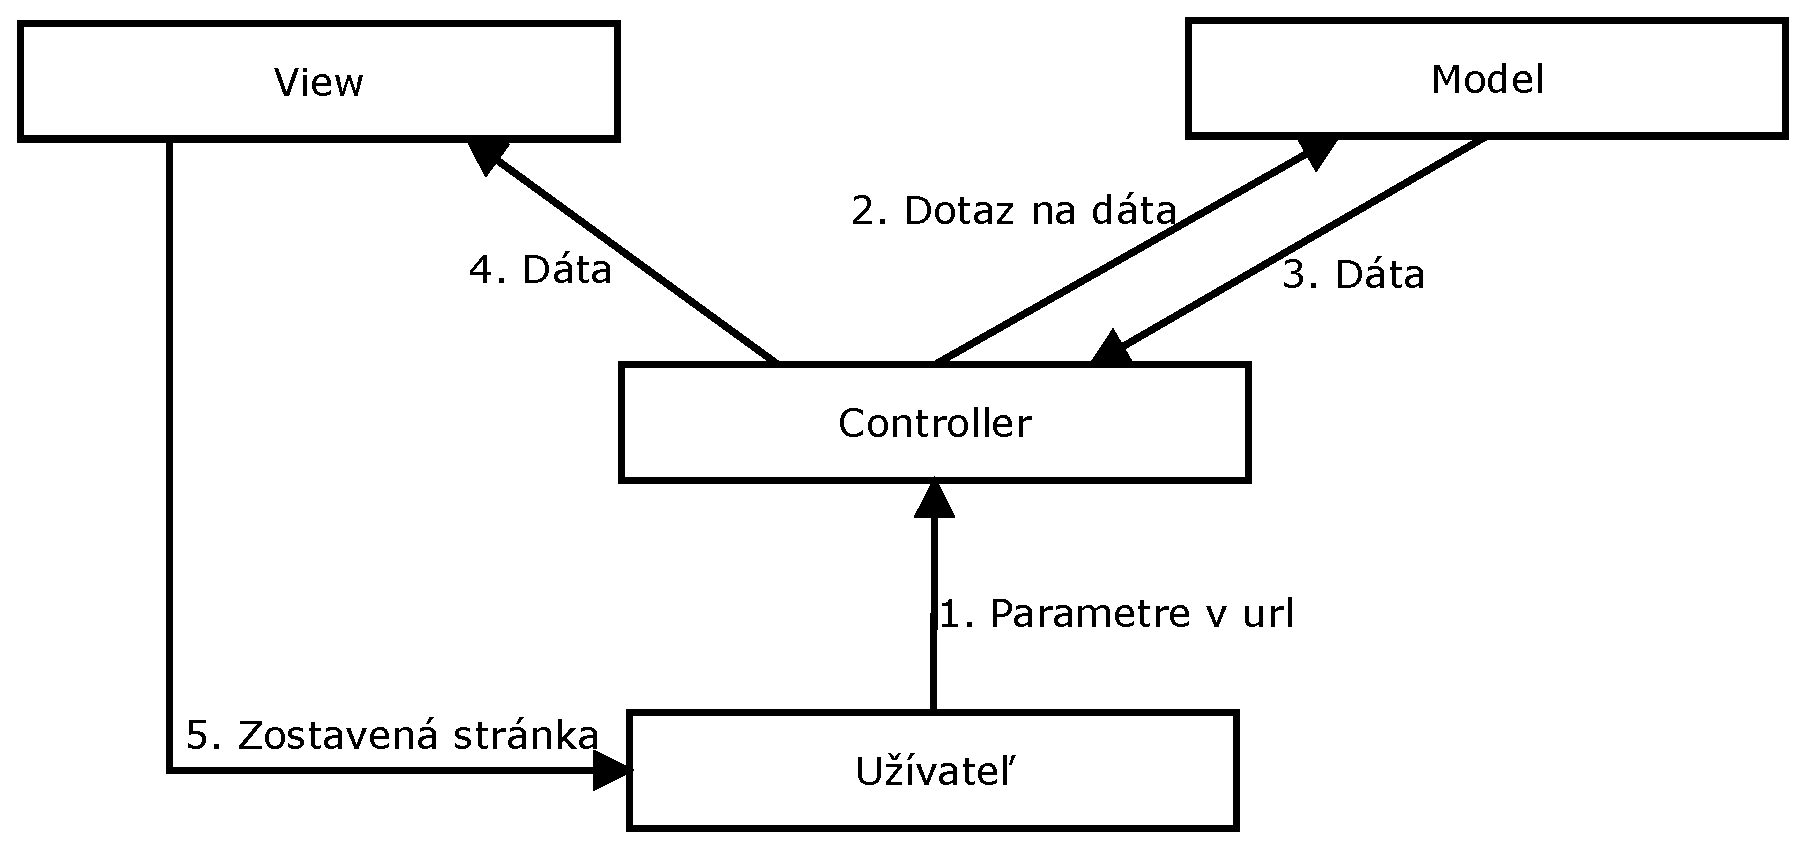
\includegraphics[scale=0.40]{fig/mvc.eps}
  \caption{Príklad MVC}
  \label{fig:mvc}
\end{figure}

\subsection{Nette}
\label{sec:nette}
PHP je síce samo o sebe mocný programovací jazyk, ale v prípade zvolenia čistého PHP, by programátor musel riešiť veľké množstvo vecí, ktoré niekto v minulosti už dávno efektívnejšie vyriešil. Okrem toho by si programátor musel dávať veľký pozor a ošetrovať početné množstvo bezpečnostných rizík. Kvôli týmto veciam bol pre účel práce vybraný aplikačný rámec Nette.

Nette je rámec napísaný v PHP5, ktorý sa zameriava na pohodlnejšie a rýchlejšie programovanie webových aplikácií a elimináciu bezpečnostných rizík. Podporuje MVC a OOP. Z veľkej časti je založený na vytváraní znovu použiteľných komponentov. K Nette patrí aj šablónovací systém Latte, ktorý zapuzdruje PHP v HTML súboroch do špeciálnych Latte makier a tým eliminuje bezpečnostné riziká. Tracy a Tester zase slúžia na hľadanie a odlaďovanie chýb. Pôvodným autorom je David Grundl, ale v súčasnosti sa o rozvoj rámcu stará Nette Foundation. Je ponúkaný pod licenciou GNU GPL a licenciou Nette (obdoba BSD licencie). Rámec sa teší veľkej obľube a taktiež početnej komunite v Čechách a na Slovensku. Minimálne požiadavky, pre správnu funkčnosť rámca, sa vyžaduje PHP verzie 5.3.1 a vyššej. Všetky požiadavky je možné overiť oficiálnym checker.php skriptom.

\section{Databázová časť}
\label{sec:databaza}
Databáza, ako prostriedok pre uloženie dát, bola zvolená hlavne kvôli vlastnosti ACID\footnote{atomickosť, konzistencia, izolovanosť a trvácnosť} a pre prístup viacerých užívateľov k databázy súčasne. Okrem iného, databázy šetria pamäťové miesto tým, že pri dobrom návrhu sa v databázy nenachádzajú redundantné dáta. Manipulácia s dátami je pomerne rýchla, pretože sa do medzi pamäte neukladá celá databáza. Nad databázou sa dajú vykonávať zložité dotazy a spájať dáta z viacerých tabuliek.  Na výber boli rôzne alternatívy ako napríklad PL/SQL, T-SQL alebo vybraný MySQL.   

\subsection{MySQL}
\label{sec:mysql}
MySQL je otvorený, viac užívateľský SQL relačný databázový server, ktorý je implementovaný vo viacerých programovacích a hlavne serverových jazykoch, napríklad v skriptovacom jazyku PHP. Je to databázový relačný systém, teda každá databáza v MySQL je tvorená z jednej alebo viacerých tabuliek, ktoré majú riadky a stĺpce. Riadky udávajú jednotlivé záznamy, stĺpce zase dátové typy jednotlivých záznamov. Práca s takouto databázou je vykonávaná pomocou takzvaných dotazov.

\section{Klientská časť}
\label{sec:klient}
Klientská časť pokrýva všetko to, čo je zobrazené užívateľovi. Teda v tomto prípade je myslená kompletná stránka, ktorej zostavovanie sa dialo z väčšej miery na servery. Aby boli informácie určené pre užívateľa zobrazené v nejakej prijateľnej a užívateľsky prívetivej podobe, tak sa vyžaduje okrem značkovacieho jazyka HTML použiť aj CSS kaskádové štýly. Keďže moderná prezentácia informácií na webových portáloch vyžaduje aj určitú ľahkosť a dynamiku, tak k tomuto účelu bol použitý celosvetovo rozšírený programovací jazyk Javascript.

\subsection{HTML}
\label{sec:html}
Hyper Text Markup Language je značkovací jazyk určený pre popis webových dokumentov, hlavne webových stránok. Najprv bol iba veľmi jednoduchá podmnožina jazyka SGML\footnote{Standard Generalized Markup Language}, ale neskôr sa z neho vyvinul samostatný štandard. HTML dokument sa popisuje pomocou HTML tagov. Každý typ HTML tagu slúži na popísanie odlišného typu obsahu dokumentu.  

V minulosti sa HTML používal na definovanie štruktúry dokumentu a aj jeho výzoru. V súčasnej dobe je HTML určené iba na zmienenú definíciu štruktúry.

\subsection{CSS}
\label{sec:css}
Kvôli tomu, že HTML sa začalo používať iba na definovanie štruktúry dokumentu a nie jeho výzoru, bol vyvinutí Cascading Style Sheets. CSS popisuje ako budú HTML tagy zobrazené na obrazovke, papieri, alebo inom médiu. CSS šetrí veľa času tým, že môže popisovať rozmiestnenie viacerých webových stránok naraz.

\subsection{Javascript}
\label{sec:javascript}
Javascript je skriptovací, prototypovo založený jazyk, ktorý sa v súčasnosti používa hlavne pri tvorbe dynamických webových prezentácií a webových stránok. Javascript beží na klientskej strane webu. Je spúšťaný väčšinou vo webových prehliadačoch. V súčasnosti Javascript podporuje väčšina webových prehliadačov a je najpoužívanejší skriptovací jazyk používaný na klientskej strane.

Bola by chyba myslieť si, že Javascript svoje uplatnenie pri tvorbe webov má iba na strane klienta. Javascript je naozaj všestranný jazyk a svoje uplatnenie nájde aj na servery napríklad v podobe Node.js. Pre účely tejto práce je avšak použitý klasický klientský Javascript spúšťaný vo webovom prehliadači.

\subsection{JQuery}
\label{sec:jquery}
JQuery je ľahká a rýchla Javascriptová knižnica, ktorej hlavným cieľom je, aby bolo použitie Javascriptu na webových stránkach omnoho jednoduchšie. Taktiež zjednodušuje komplikované veci Javascriptu, ako AJAX volania a manipuláciu s DOM. Okrem toho obsahuje metódy na manipuláciu s CSS, HTML udalosti, efekty a animácie a ďalšie nápomocné programy. Je rozšíriteľná pomocou pluginov a na väčšinu známych vecí už existuje JQuery plugin. Knižnica zároveň rieši tzv. cross-browser problémy, kedy jedna vec sa môže v rôznych prehliadačoch správať odlišne.

Je to najobľúbenejšia a najrozšírenejšia Javascriptová knižnica, čomu dáva za pravdu nielen početná komunita okolo, ale aj to, že je využívaná najväčšími firmami ako Google, či Microsoft.

\subsection{Bootstrap}
\label{sec:bootstrap}
Bootstrap je frontendový aplikačný rámec pre rýchle a ľahké vyvíjanie responzívnych webových stránok. Obsahuje predpripravené dizajnérske typografické šablóny založené na HTML a CSS. Hodí sa predovšetkým na prototypovanie, hlavne kvôli značnej neoriginalite vytvorených stránok, keďže väčšina stránok založená na tomto rámci vypadá veľmi podobne. Na druhú stranu, jednoduchými modifikáciami si môže skúsený dizajnér upraviť Bootstrap k svojmu obrazu.   

\subsection{Chart.js}
\label{sec:chartjs}
Chart.js je ľahká Javascriptová knižnica, pomocou ktorej je tvorba grafov z daných dát veľmi jednoduchá. Na zobrazovanie grafov používa HTML tag <canvas > do ktorého sa grafy vykresľujú. Na výber je z 6 najbežnejších typov grafov. Takto vytvorené grafy sú plne responzívne, takže môžu byť správne zobrazené, ako na stolných počítačoch s veľkou obrazovkou, tak aj na malých mobilných zariadeniach.

\section{API}
\label{sec:api}
API je v tomto prípade myslené, ako knižnica, pomocou ktorej vývojári hier pristupujú k funkciám webovej platformy. Knižnica je implementovaná v Javascripte a k funkciám platformy, ktoré sú implementované na servery sa pristupuje pomocou dotazovaním technológiou AJAX.

\subsection{AJAX}
\label{sec:ajax}
Asynchronous Javascript and XML je súhrnné označenie technológií, ktoré umožňujú meniť obsah webových stránok bez nutnosti znovu načítania celej stránky zo servera. Hlavná výhoda spočíva v tom, že sa prenáša značne menšie množstvo dát. AJAX nie je samostatný programovací jazyk, ani technológia sama o sebe, ako by sa mohlo zdať. Je to skôr kombinácia niekoľkých prvkov. Je založený na internetových štandardoch. Používa kombináciu HMLHttpRequest pre získanie dát zo servera a Javascript/DOM pre zobrazenie a použitie dát.
\begin{figure}[h]
  \centering
  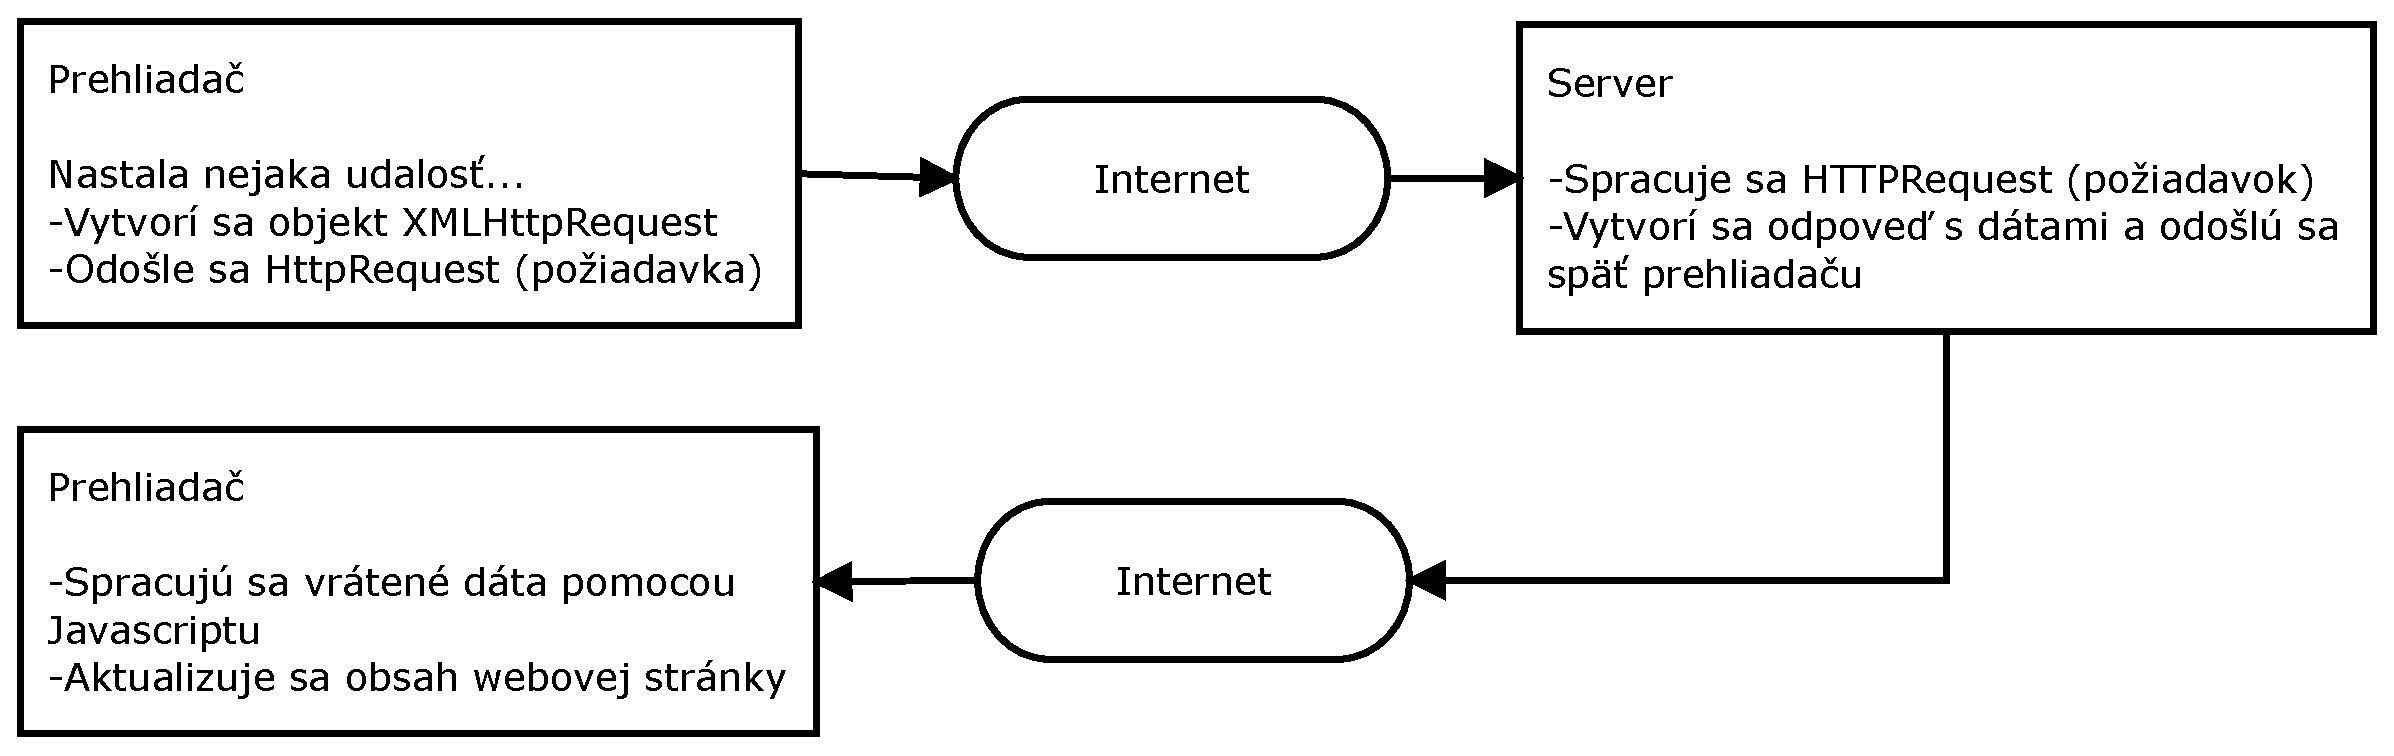
\includegraphics[scale=0.40]{fig/ajax.eps}
  \caption{Neblokujúca komunikácia so serverom pomocou AJAXu}
  \label{fig:ajax}
\end{figure}

\subsection{CORS}
\label{sec:cors}
Klasický Javascript je limitovaný tzv. Same origin policy. Z toho dôvodu nie je možné prijímať odpovede na dotazy z domény inej, ako je doména z ktorej bola požiadavka vyslaná.

Tento známy, hore popísaný problém rieši Cross-origin resource sharing. CORS je vlastne mechanizmus, ktorý povoľuje zakázané zdroje na webovej stránke, a tak je možné prijímať odpovede na požiadavky z inej domény, ako z domény z ktorej zdroje pochádzajú. Pre použitie tohto mechanizmu musí nastať zmena pri tvorbe požiadavku na klientovi a tiež je treba povoliť CORS na servery. Prehliadač musí posielať nastavenie Origin: doména v HTTP hlavičke. Na servery zase musí byť nastavené povolenie Acces-Control-Allow-Origin: doména, alebo * pre povolenie všetkých domén.

\section{Hra}
\label{sec:hra}
Pre demonštračnú hru sa ponúkalo buďto použiť klasický Javascript, čo ale nie je príliš rozšírená forma tvorby Javascript/HTML5 hier, alebo použiť jeden z početného množstva aplikačných rámcov, ktoré sú určené špeciálne na tvorbu hier. Na výber bol Ease.js, Tree.js, Panda.js, melon.js, Kiwi.js, alebo Phaser.js a mnoho ďalších. Bol vybraný Phaser.js, pretože to je jeden z najpoužívanejších a najbežnejších Javascriptových rámcov určených pre programovanie hier, o čom svedčí hlavne početná komunita okolo tohto rámca a fakt, že aj mnohé firmy z oblasti herného biznisu, ako Boostermedia, pracujú práve s týmto rámcom. 

\subsection{Phaser}
\label{sec:phaser}
Phaser je Javascriptový aplikačný rámec určený špeciálne pre tvorbu hier, ako desktopových, tak aj mobilných. Je založený na renderovacom rámci pixi.js. Phaser je ľahko osvojiteľný, rýchly, je ponúkaný zadarmo a má otvorený kód. Podporuje canvas a zároveň aj webgl. Obsahuje veľké množstvo predpripravených funkcií. Tieto funkcie sú spracované tak, aby ich použitie bolo jednoduché. Príkladom môže byť stavaný preloader, fyzika, animácie, častice, rôzne módy prispôsobenia veľkosti obrazovky a iné.  

%%%%%%%%%%%%%%%%%%%%%%%%%%%%%%%%%%%%%%%%%%%%%%%
\chapter{Analýza existujúcich riešení}
\label{chap:analyza}
V tejto kapitole budú predstavené konkurenčné, existujúce a predovšetkým známejšie riešenia určené zväčša pre iné platformy, ako je platforma, pre ktorú je riešenie tejto práce určené. Určite existuje oveľa viac alternatív, ale vymenúvať a rozobrať všetky nie je účelom tejto práce.

\section{Steam}
Steam je herná platforma od spoločnosti Valve Corporation určená predovšetkým k digitálnej distribúcií hier a vytvoreniu komunity hráčov týchto hier. Steam klient je podporovaný na rôznych platformách. Na počiatku podporoval iba platformu Windows, neskôr svoje pôsobenie rozšíril na platformu Mac a nakoniec na Linuxové distribúcie. Pochopiteľne nie všetky hry nachádzajúce sa na Steam platforme sú hrateľné vo všetkých operačných systémoch. Momentálne samotná platforma obsahuje viac ako 3500 hier a teší sa početnej komunite hráčov.

Pre možnosť distribúcie hry na Steam je vývojár nútený si zakúpiť prístup k službe Steam Greenlight, ktorý stojí v dobe vzniku tejto práce 90 EUR. Poplatok je jednorazový a vývojár nie je obmedzený počtom publikovaných hier v tejto službe. Po publikovaní hry v službe Steam Greenlight sa avšak hra nenachádza ešte na samotnej platforme. Užívatelia vďaka tejto službe môžu hlasovať za hru a hra sa na platformu Steam dostáva až po získaní určitého počtu hlasov. Je teda na samotnom vývojárovi vynaložiť úsilie, aby bola hra čo najlepšie spropagovaná a všimol si ju a samozrejme aj hlasoval čo možno najväčší počet oslovených ľudí. 

Steam pre vývojárov hier, ktorých hry boli schválené komunitou Steam Greenlight pre možnosť distribúcie hry na platforme, ponúka svoje Steamworks API. Steamworks API dovoľuje vývojárom hier integrovať rôzne funkcie ako štatistiky, odmeny, autentifikácia, tvorba zápasov, peer-to-peer networking, Steam cloud úložisko, Valve anticheat\footnote{Software, ktorý slúži ako prevencia proti neférovému získaniu výhody v online hre pomocou softwaru tretích strán}, hlasový chat a v neposlednej rade aj DRM\footnote{Digital rights management - metódy, ktorých účelom je kontrolovať používanie obsahu digitálnych médií}. Všetky tieto funkcie je možné dohľadať na oficiálnej stránke Steamworks API.
\begin{figure}[h]
  \centering
  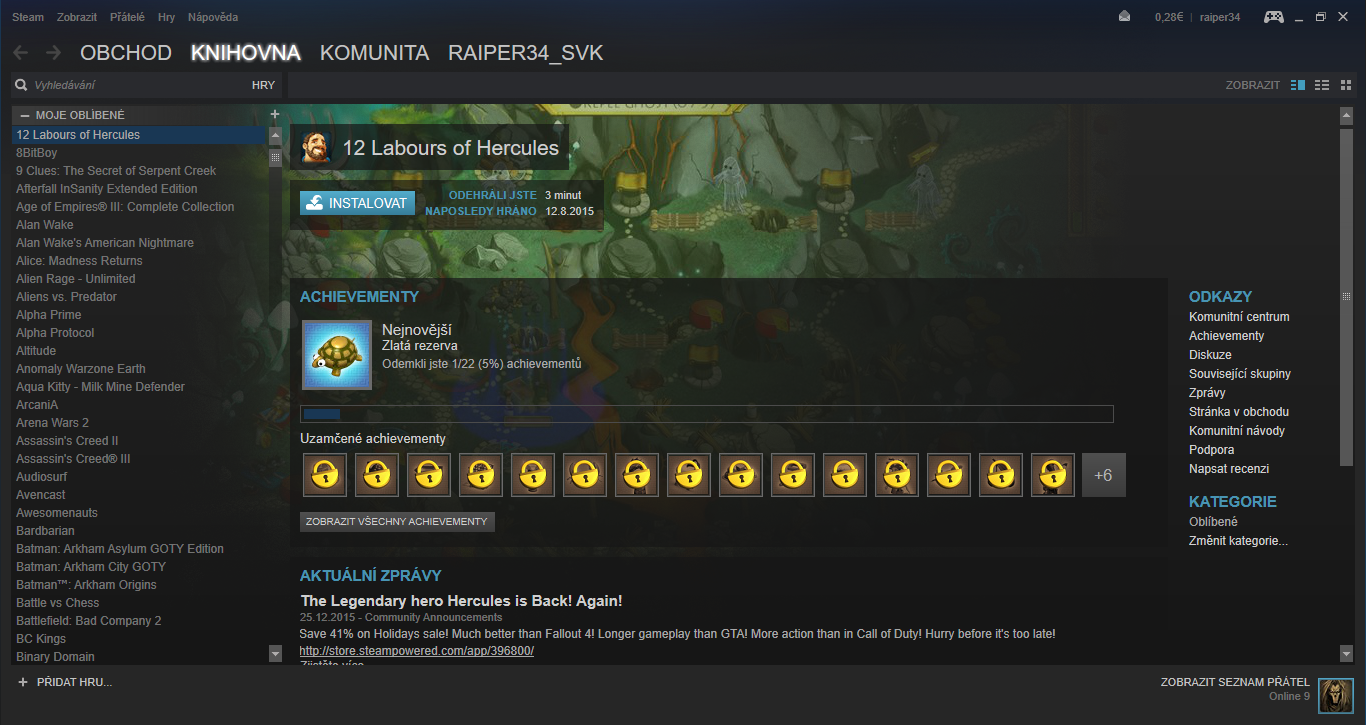
\includegraphics[scale=0.27]{fig/steam.png}
  \caption{Ukážka steam klienta na Windows}
  \label{fig:steam}
\end{figure}

\section{Google Play Game Services}
Po predstavení operačného systému Android vyvinul Google svoj internetový obchod Google Play, ktorý ponúka nielen aplikácie a hry pre Android, ale po novom aj knihy hudbu a filmy. Vývojári momentálne môžu získať prístup na publikovanie aplikácií  v tomto obchode za poplatok 20USD, ktorý sa platí jednorazovo, pričom reálne nie sú limitovaný počtom aplikácií a ani kvalitou výslednej publikovanej aplikácie.

Okrem toho, Google dáva možnosť vývojárom hier integrovať do ich diel svoje Play Game Services API. Zprvu bolo API limitované iba na Android hry, v súčasnosti avšak podporuje už aj webové aplikácie. Pred samotným použitím API si vývojár musí najprv definovať hru v Google Play Developer Console a poprípade ďalšie doplnkové funkcie, ktoré chce integrovať a využívať. API ponúka možnosti použitia odmien, skóre tabuliek, multiplayeru, uloženia dát v cloude, udalosti, úlohy a iné. Ďalšie informácie sú k nájdeniu v oficiálnej dokumentácií.   
\begin{figure}[h]
  \centering
  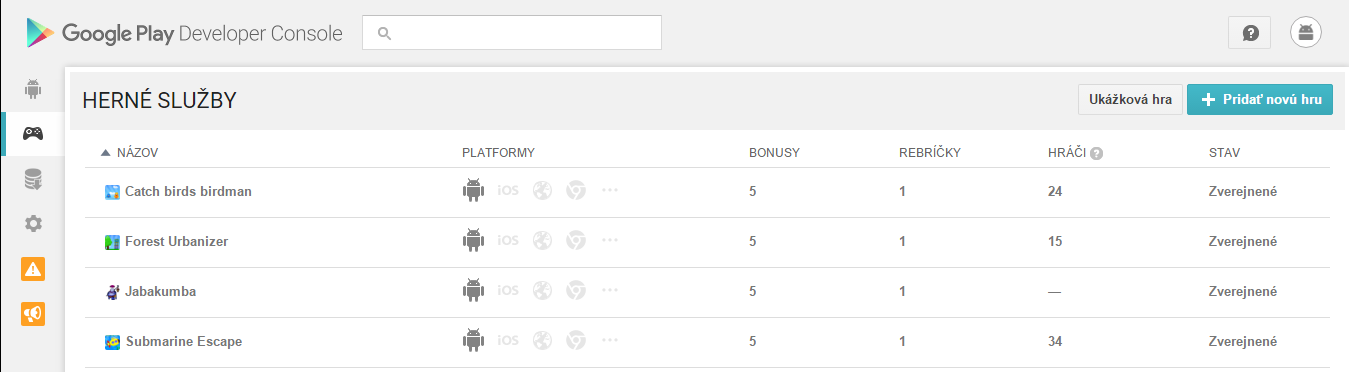
\includegraphics[scale=0.32]{fig/google-play.png}
  \caption{Ukážka Google Play Developer Console  - zoznam existujúcich hier}
  \label{fig:google-play}
\end{figure}

\section{Apple Game Center}
Rovnako ako Google má pre Android svoj internetový obchod s Android aplikáciami, tak aj Apple má svoj App Store s aplikáciami pre svoje zariadenia. Na rozdiel od Google Play, vývojár pre prístup do App Store musí platiť ročne buď 99 USD za Apple Developer Program, alebo 299 USD za Apple Developer Enterprise Program. Viac informácií, ako aj rozdiely v týchto programoch, je možné nájsť na oficiálnej stránke Apple.  

Apple tiež ponúka svoje Game Center API. API je integrovateľné do iOS hier a taktiež do OS X. Game Center umožňuje integrovať skóre tabuľky, odmeny, pozývanie priateľov do hry a spúšťanie multiplayer hier pomocou systému automatického vytvárania hier\footnote{Matchmaking}.

\section{Facebook Game Services}
Za zmienku určite stojí aj najväčšia a najpopulárnejšia sociálna sieť Facebook, ktorá od svojho vzniku v roku 2004 pridala nespočetné množstvo vylepšení, medzi ktorými sa objavili aj hry. V tomto momente to už zďaleka nie je len sociálna sieť, ako by sa mohlo na prvý pohľad zdať. Vývojári majú tak možnosť na tejto sociálnej sieti publikovať svoje hry a dokonca integrovať špeciálne funkcie ponúkané vývojárom vďaka Facebook Game Services API. API je integrovateľné do širokého spektra platforiem a enginov od Flash a HTML5 hostovaných na Facebooku, ktoré sú možné nájsť v Facebook App Store, až po mobilné hry platformy Android a iOS. API štandardne ponúka odmeny, skóre tabuľky a štatistiky + ďalšie rozširujúce funkcie sociálnej siete zahrnujúc zdieľanie na nástenke profilu užívateľa, alebo notifikácie. Záznam hry nachádzajúcej sa v Facebook App Store môžete vidieť na obrázku \ref{fig:facebook}.
\begin{figure}[h]
  \centering
  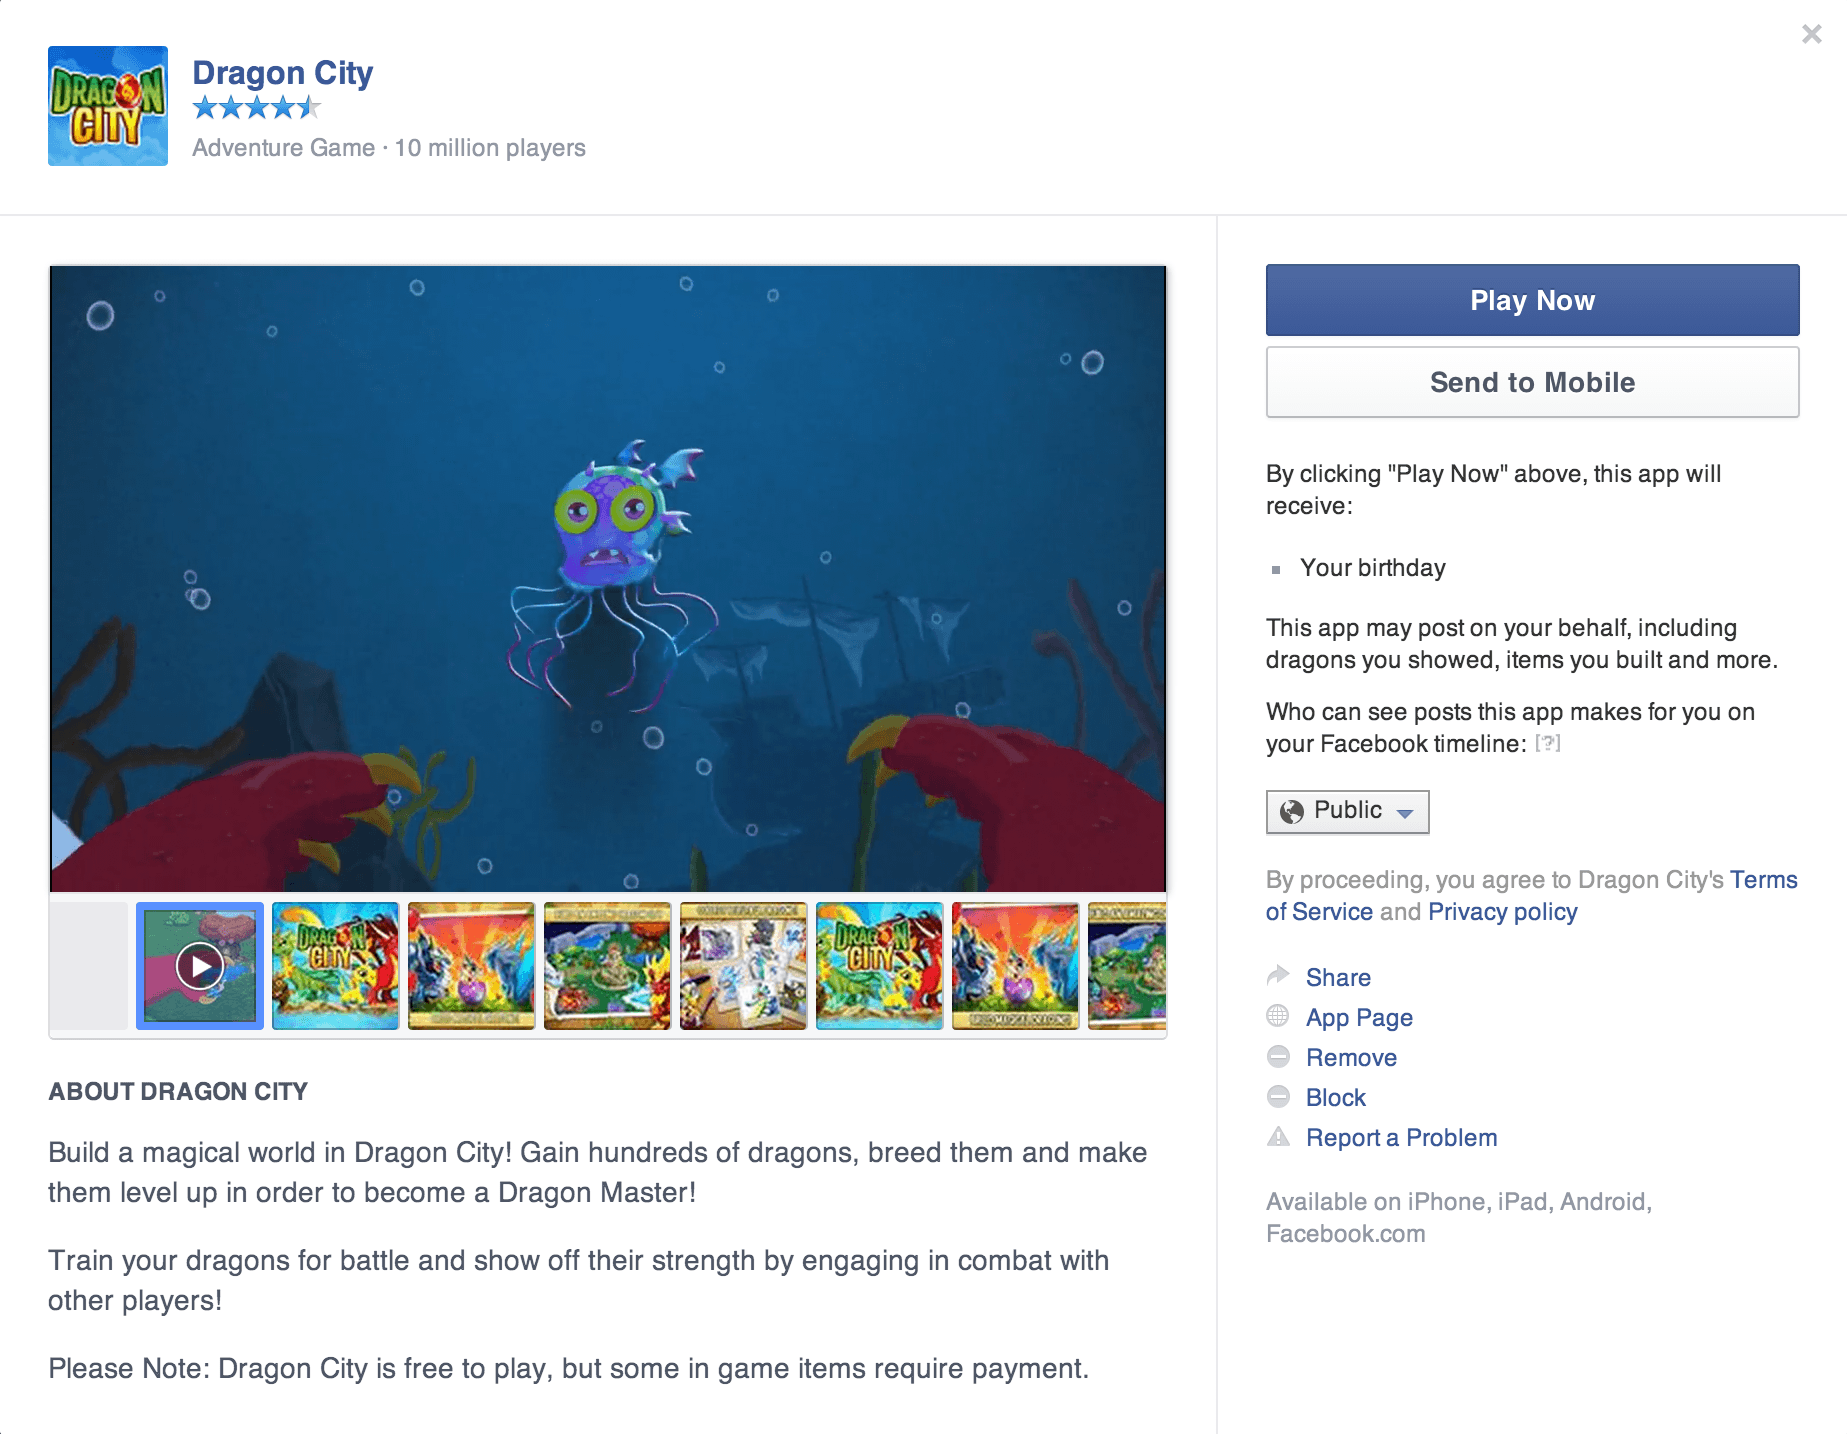
\includegraphics[scale=0.17]{fig/facebook.png}
  \caption{Záznam hry v Facebook App Store}
  \label{fig:facebook}
\end{figure}

\section{Clay.io}
Clay.io je webový projekt zameraný na Javascript/HTML5 hry, ktorý vytvoril v roku 2012 Austin Hallock. Z prvu bol tento projekt rovnomerne orientovaný, ako na vývojárov hier, tak aj na hráčov týchto hier. Hry mohli byť na platforme hostované zadarmo. Platforma neobsahovala žiadne kvalitatívne obmedzenia čo sa týka uverejňovania hier a jej služby boli zadarmo. Bolo možné do hry integrovať vlastné Javascriptové API, ktoré sprístupňovalo skóre tabuľky, odmeny, cloud úložisko dát, cross promotion\footnote{Forma propagácie, kedy je zákazníkom jednoho preduktu predstavovaný podobne zameraný produkt}, reklamy tretích strán. Okrem toho na základe už vložených informácií Clay.io dokázalo generovať rôzne konfiguračné súbory pre webové obchody ako Chrome Web Store, alebo Firefox Marketplace. Začiatkom roka 2015 sa avšak situácia zmenila a Clay.io sa uzavrelo. Začalo sa orientovať na vyššiu kvalitu hier a k API už mohli pristupovať iba oprávnení schválení vývojári. Publikovať hry s takýmto API bolo po novom tiež možné iba na webe Clay.io a v špeciálnej Clay.io aplikácií, ktorá je určená pre Android, poprípade na ďalších weboch, alebo v aplikáciách, avšak iba na tých pár vybraných. s ktorými Clay.io spolupracuje.    

\section{Ostatné}
Pre webové hry postavené na technológií Flash existovalo a stále ešte existuje hneď niekoľko herných portálov určených predovšetkým pre hráčov, ktoré ale taktiež ponúkajú vývojárom možnosť integrovať rôzne služby konkrétneho webového portálu do hry. Príkladom môže byť zaniknutý Mochimedia, alebo stále existujúce herné webové portály Newgrounds.com, Gamejolt.com, alebo Kongregate.com. Nevýhodou týchto portálov je to, že použitie ich API, je často limitované iba na použitie na danom webovom portáli. Všetky zmienené portáli ponúkali, alebo stále ponúkajú obdobné funkcie API, ako tomu bolo v predchádzajúcich častiach. 
\begin{figure}[h]
  \centering
  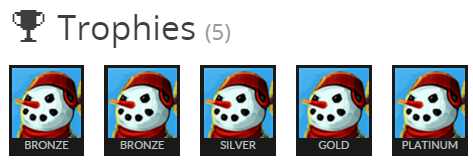
\includegraphics[scale=0.5]{fig/odmeny2.png}
  \caption{Ukážka odmien na stránke Gamejolt.com}
  \label{fig:odmeny}
\end{figure}

Boli vymenované riešenia asi pre takmer všetky webové, desktopové a mobilné platformy. Je ale nutné podotknúť, že herné konzoly tiež nezostávajú pozadu a taktiež obsahujú väčšinu z vymenúvaných komponent, čo je samozrejme prirodzené, keďže tieto komponenty často pridávajú hre na atraktivite. Dobrým zástupcom je Xbox, alebo Playstation. Avšak možnosti stredných, vôbec neuvažujúc malých, herných štúdií a vývojárov, ktorý chcú na týchto platformách publikovať sú dosť obmedzené, keďže sú akceptované poväčšine iba veľké AAA tituly\footnote{V hernom premysle označuje herné tituly, s najväčším rozpočtom, levelom propagácie, alebo s najvyšším hodnotením od kritikov} a keď Indie hry\footnote{Nezávislá hra vyvíjaná bez finančnej podpory vydavateľa}, tak naozaj veľmi kvalitné, alebo populárne.

%%%%%%%%%%%%%%%%%%%%%%%%%%%%%%%%%%%%%%%%%%%%%%%
\chapter{Návrh riešenia}
\label{chap:navrh}
Táto kapitola popisuje návrh riešenia tejto bakalárskej práce. Najprv pojednáva o analýze požiadaviek na komponenty, ktoré sú zahrnuté v API a na celkovú štruktúru webovej platformy. Kapitola ďalej popisuje návrh webovej platformy z hľadiska funkcionality a následne z hľadiska grafického užívateľského rozhrania. Hneď nato nasleduje návrh databáze a je predstavený jej konceptuálny model. Na konci kapitoly je predstavený návrh samotného API a návrh jednoduchej HTML5 hry, ktorá má za úlohu demonštrovať funkcie tohto API.  

\section{Analýza požiadaviek na komponenty}
Požiadavky na komponenty čiastočne vychádzajú z predchádzajúcej kapitoly o Analýze už existujúcich riešení. Boli vybrané komponenty z daných existujúcich riešení také, ktoré sa najviac opakovali v daných službách, teda boli v určitom zmysle žiadané, a ktoré boli reálne použiteľné na tvorenej webovej platforme. Okrem toho bol zostavený orientačný doplňujúci dotazník, cielený práve na vývojárov hier a špeciálne na vývojárov webových html5 hier. Dáta boli zberané na fórach\footnote{http://www.html5gamedevs.com/, https://www.scirra.com/forum/}, kde sa združujú vývojári takýchto hier a v špeciálnych skupinách sociálnych sietí\footnote{HTML5 Mobile Game and App Development a Game Development Community CZ/SK na Facebooku}, ktoré obsahujú takto odborovo orientovaných ľudí. V dotazníku odpovedalo 47 ľudí. Títo ľudia mali vybrať 3 komponenty, ktoré pokladajú pre seba ako vývojárov za najužitočnejšie. Pritom bolo jedno z akého hľadiska, či z hľadiska toho, že komponenta má obohacovať hru napríklad o tabuľku skóre, či odmeny a tak jej pridávať na atraktivite, alebo naopak má slúžiť skôr vývojárovi ako napríklad štatistiky prístupov, alebo kontrola domény, na ktorej sa daná hra nachádza. Výsledky môžete vidieť na obrázku \ref{fig:dotaznik}. Dáta slúžia iba pre predstavu, čo najviac vývojárom chýba, alebo naopak, ktoré komponenty z vymenúvaných pokladajú z ich hľadiska za najdôležitejšie, najprínosnejšie.  

Na základe tohto dotazníku, ale predovšetkým na základe analýzy už existujúcich riešení bola vybraná nasledujúca množina komponent.
\begin{enumerate}
\item Tabuľky skóre
\item Odmeny
\item Kontrola domén
\item Štatistiky prístupov
\item Úložisko v cloude
\end{enumerate}
Niektoré komponenty neboli vybrané z dôvodu, že neboli pokladané vývojármi za až tak podstatné (napríklad cross-promotion), alebo sa nehodili k danému projektu (napríklad chat, ktorý by v hre na mobilných zariadeniach s nie až tak veľkými obrazovkami, mohol byť viac na obtiaž, než k úžitku). Ďalšia komponenta, s ktorou sa v tomto projekte nepočíta, aj keď v dotazníku bola táto možnosť pomerne chcená, je integrácia reklám do hry. Takáto komponenta by bola nad rámec tejto práce a muselo by sa okolo nej riešiť niekoľko ďalších vecí, ako je získanie inzerentov, správa reklamných kampaní a ďalšie z väčšej miery netechnické veci.
\begin{figure}[h]
  \centering
  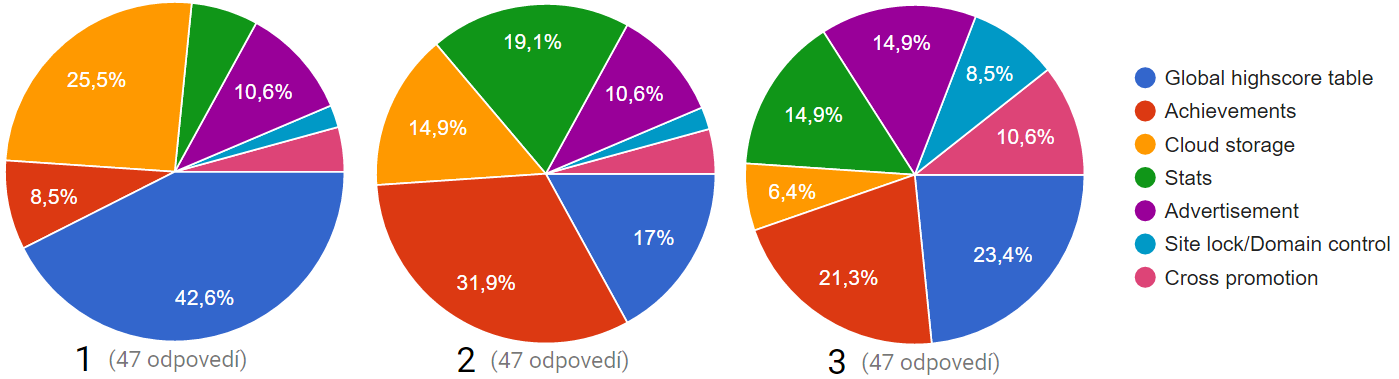
\includegraphics[scale=0.4]{fig/graf-dotazniku.png}
  \caption{Výsledky dotazníku}
  \label{fig:dotaznik}
\end{figure}

\section{Návrh webovej platformy}
Návrh webovej platformy bol vypracovávaný po analýze existujúcich herných platforiem, herných klientov a webových portálov, ktoré sú čiastočne uvedené v kapitole 3. V prvom rade bolo treba premyslieť, k čomu všetkému by mala daná webová platforma slúžiť, čo všetko by na nej malo byť realizovateľné, aké možnosti by ponúkala pre vývojárov hier, a aké možnosti zase pre hráčov týchto hier.

Tento návrh, toho, čo všetko môže daný užívateľ so svojou rolou na portáli vykonávať bol spracovaný pomocou Use Case Diagramu (Diagramu prípadov užitia) ďalej iba UCD, ktorý zobrazuje chovanie systému, tak ako ho vidí užívateľ. Účelom tohto diagramu je popísať funkcionalitu systému, teda čo sa od systému očakáva. Diagram hovorí o tom, čo má systém, v tomto prípade naša webová platforma, vedieť, ale nehovorí už o tom, ako sa to bude vykonávať. UCD sa skladá z prípadov užitia (Use Case), aktérov (Actor) a vzťahov medzi nimi. Prípad užitia je sada niekoľkých akcií, ktoré vedú k dosiahnutiu určitého cieľa. Aktér je rola, ktorá komunikuje s jednotlivými prípadmi užitia. Zjednodušene povedané UCD je diagram, ktorý zobrazuje to, čo všetko daná užívateľská rola môže v systéme vykonávať. Na obrázku \ref{fig:ucd} môžete vidieť naľavo aktéra a napravo prípad užitia.
\begin{figure}[h]
  \centering
  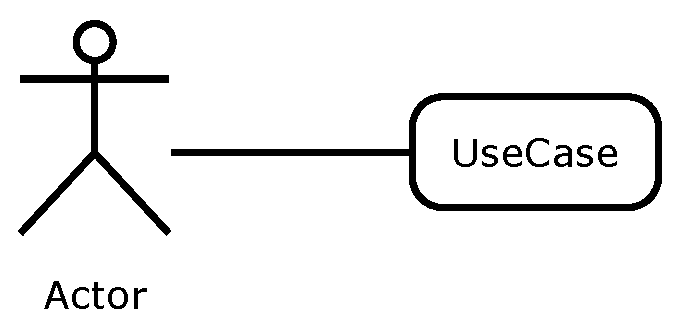
\includegraphics[scale=0.43]{fig/ucd.eps}
  \caption{Use Case Diagram, naľavo aktér, napravo prípad užitia}
  \label{fig:ucd}
\end{figure}

Prvou rolou, ktorou sa užívateľ stáva po príchode na webovú platformu je rola neprihláseného návštevníka. Prirodzene neprihlásený návštevník musí mať obmedzenú množinu toho, čo môže na danej stránke vykonávať. V prípade tejto bakalárskej práce môže byť neprihlásený užívateľ napríklad hráč, ktorý sa ešte nezaregistroval, alebo sa z nejakého dôvodu nechce registrovať. Na portál prišiel vyložene skrátiť si nejakú nudnú chvíľu, skóre tabuľky najlepších hráčov ho nemotivujú k súťaženiu s ostatnými hráčmi a ani odmeny nepokladá za motivujúci prvok hry. Keďže platforma by mala byť optimalizovaná pre prenosné zariadenia ako mobily a tablety, tak to môže byť hráč s mobilným zariadením čakajúci napríklad v ordinácií lekára, alebo na autobusovej zastávke. Takýto hráč teda potrebuje jediné. Potrebuje zobraziť zoznam hier, aby si vybral hru, ktorú chce hrať a prípadne potrebuje filtrovať zoznam hier podľa nejakých kategórií, ako napríklad žánru a podobne. Po vybraní hry si chce prečítať nejaké základné informácie o hre, inštrukcie ako hru ovládať a v neposlednom rade náhľady, alebo iné grafické materiály, pochádzajúce najlepšie priamo z danej hry. Po tom všetkom chce samozrejme daný hráč hrať samotnú hru umiestnenú na portáli. Neprihláseným návštevníkom môže byť avšak aj hráč, ktorý sa chce na daný portál prihlásiť, poprípade sa zaregistrovať a mať tak možnosť využívať všetku funkcionalitu daného portálu, určenú pre rolu prihláseného hráča. Posledným prípadom, ktorý môže vystupovať  ako neprihlásený návštevník je, užívateľ, ktorý chce na tomto portáli získať rolu vývojára hry a mať tak možnosť sa podieľať na tvorbe herného obsahu, alebo využívať iné funkcie určené vývojárom. Diagram prípadov užitia, ktorý zhrnuje tento odsek je na obrázku \ref{fig:ucdneprihlaseny}.
\begin{figure}[h]
  \centering
  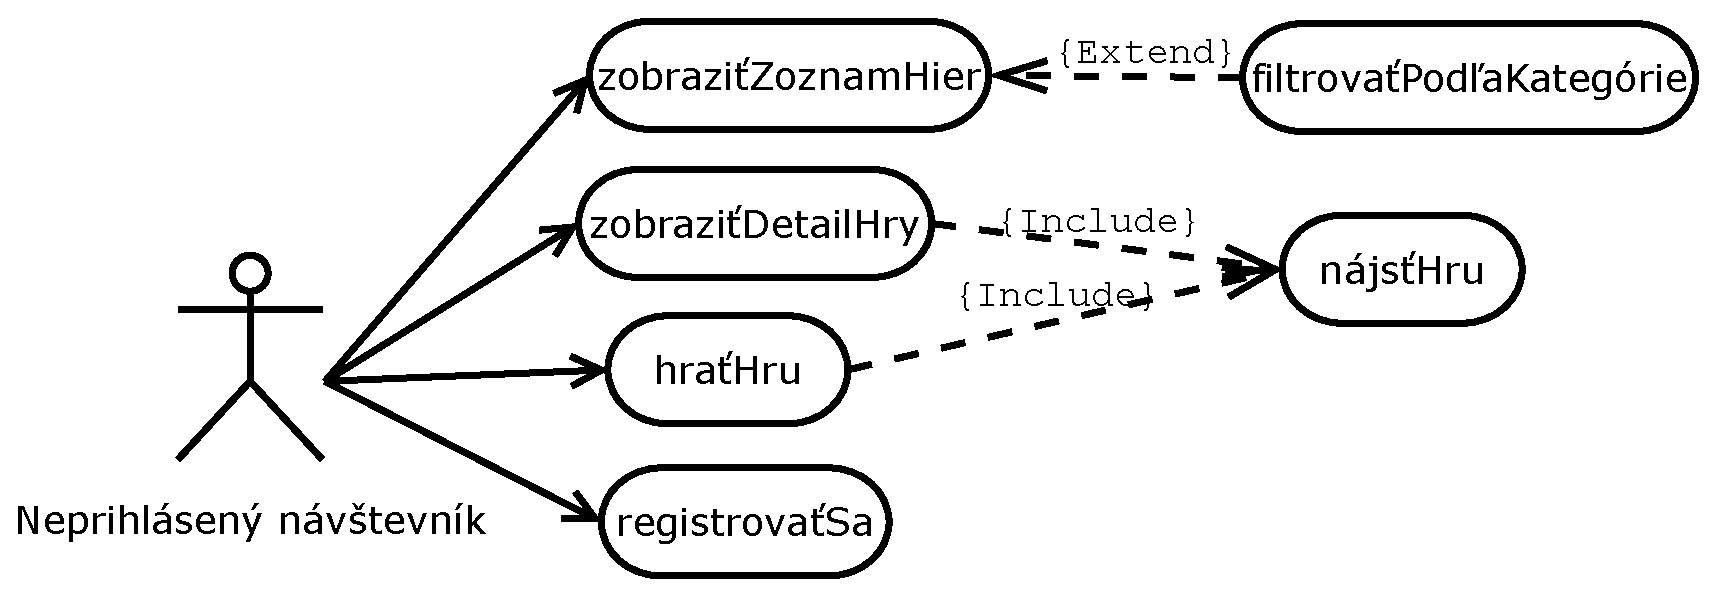
\includegraphics[scale=0.43]{fig/ucd-neprihlaseny.eps}
  \caption{Use Case Diagram neprihláseného užívateľa}
  \label{fig:ucdneprihlaseny}
\end{figure}

V poradí druhou rolou ktorou sa užívateľ môže stať v rámci systému je rola prihláseného hráča. Neprihlásený návštevník sa prihláseným hráčom stáva od chvíle, kedy sa prihlási k svoju účtu hráča.  Prihlásený hráč môže vykonávať na portáli všetky akcie, ktoré môže vykonávať rola neprihláseného návštevníka, teda zobrazovať zoznam hier, filtrovať ich, zobrazovať detaily o hre a hrať hru. K tomu ešte môže vykonávať ďalšie akcie, na ktoré je potrebné byť prihlásený. Prihlásený hráč môže hrať hry pod svojim účtom. Tým pádom môže hráč získavať v danej hre odmeny a umiestňovať sa v skóre tabuľkách najlepších hráčov a tým nepriamo súťažiť s ďalšími prihlásenými hráčmi. Okrem toho, prihlásený hráč má možnosť číselne ohodnotiť hru, alebo zdieľať svoje pocity z hry s ostatnými , publikovaním svojho komentáru na stránke s hrou. Hráč by mal mať možnosť tiež prezerať si svoj hráčsky profil a profil ostatných hráčov. Use case diagram, ktorý popisuje akcie prihláseného hráča môžete vidieť na obrázku \ref{fig:ucdprihlasenyhrac}.
\pagebreak
\begin{figure}[h]
  \centering
  \includegraphics[scale=0.43]{fig/ucd-prihlasenyhrac.eps}
  \caption{Use Case Diagram prihláseného hráča}
  \label{fig:ucdprihlasenyhrac}
\end{figure}

Treťou a asi aj najvýznamnejšou rolou v rámci tejto práce je rola vývojára. Užívateľ rolu vývojára nadobudne zaregistrovaním/prihlásením sa do svojho vývojárskeho účtu. Vývojár má povolené vykonávať to isté, ako predošlé dve role, neprihlásený návštevník a zároveň prihlásený hráč. V pomyslenej hierarchií je táto rola zase o niečo vyššie, ako spomenuté predošlé dve. Rola vývojára je schopná vytvárať a definovať nové hry, editovať informácie o hre, či už existujúcej, alebo novo vytváranej. Vývojár ďalej musí byť schopný nahrať herné súbory, obrázky k hre, ikony a iné promočné materiály potrebné pre platformu. Musí byť schopný zatiaľ nepublikovanú hru publikovať/poslať na schválenie a už publikovanú hru odstrániť zo zoznamu hier viditeľných pre neprihláseného návštevníka a prihláseného hráča. Ďalej tento užívateľ, ktorý pracuje pod touto rolou musí byť schopný zobraziť štatistiky prístupov o hre, poprípade zmeniť typy zobrazovaných štatistických grafov. Jednou z najvýznamnejších funkcií portálu, ku ktorej má táto rola prístup je práca s API. Presnejšie sa jedná od definovanie API komponent, ktoré boli popísané v kapitole 3. Táto práca s API zahrňuje definovanie, vytváranie nových odmien, editovanie už existujúcich a taktiež možnosť ich odstránenia. Umožňuje prácu s tabuľkami skóre, ich definovanie, vytváranie, editovanie, odstránenie, ich rôzne nastavenia... Tiež umožňuje definovať cloud úložisko, editovať ho, alebo ho kompletne odstrániť. V neposlednom rade by mal byť vývojár schopný definovať na ktorej doméne je možné hru s API spustiť a na ktorej nie, poprípade túto funkcionalitu vypnúť/zapnúť. 
\begin{figure}[h]
  \centering
  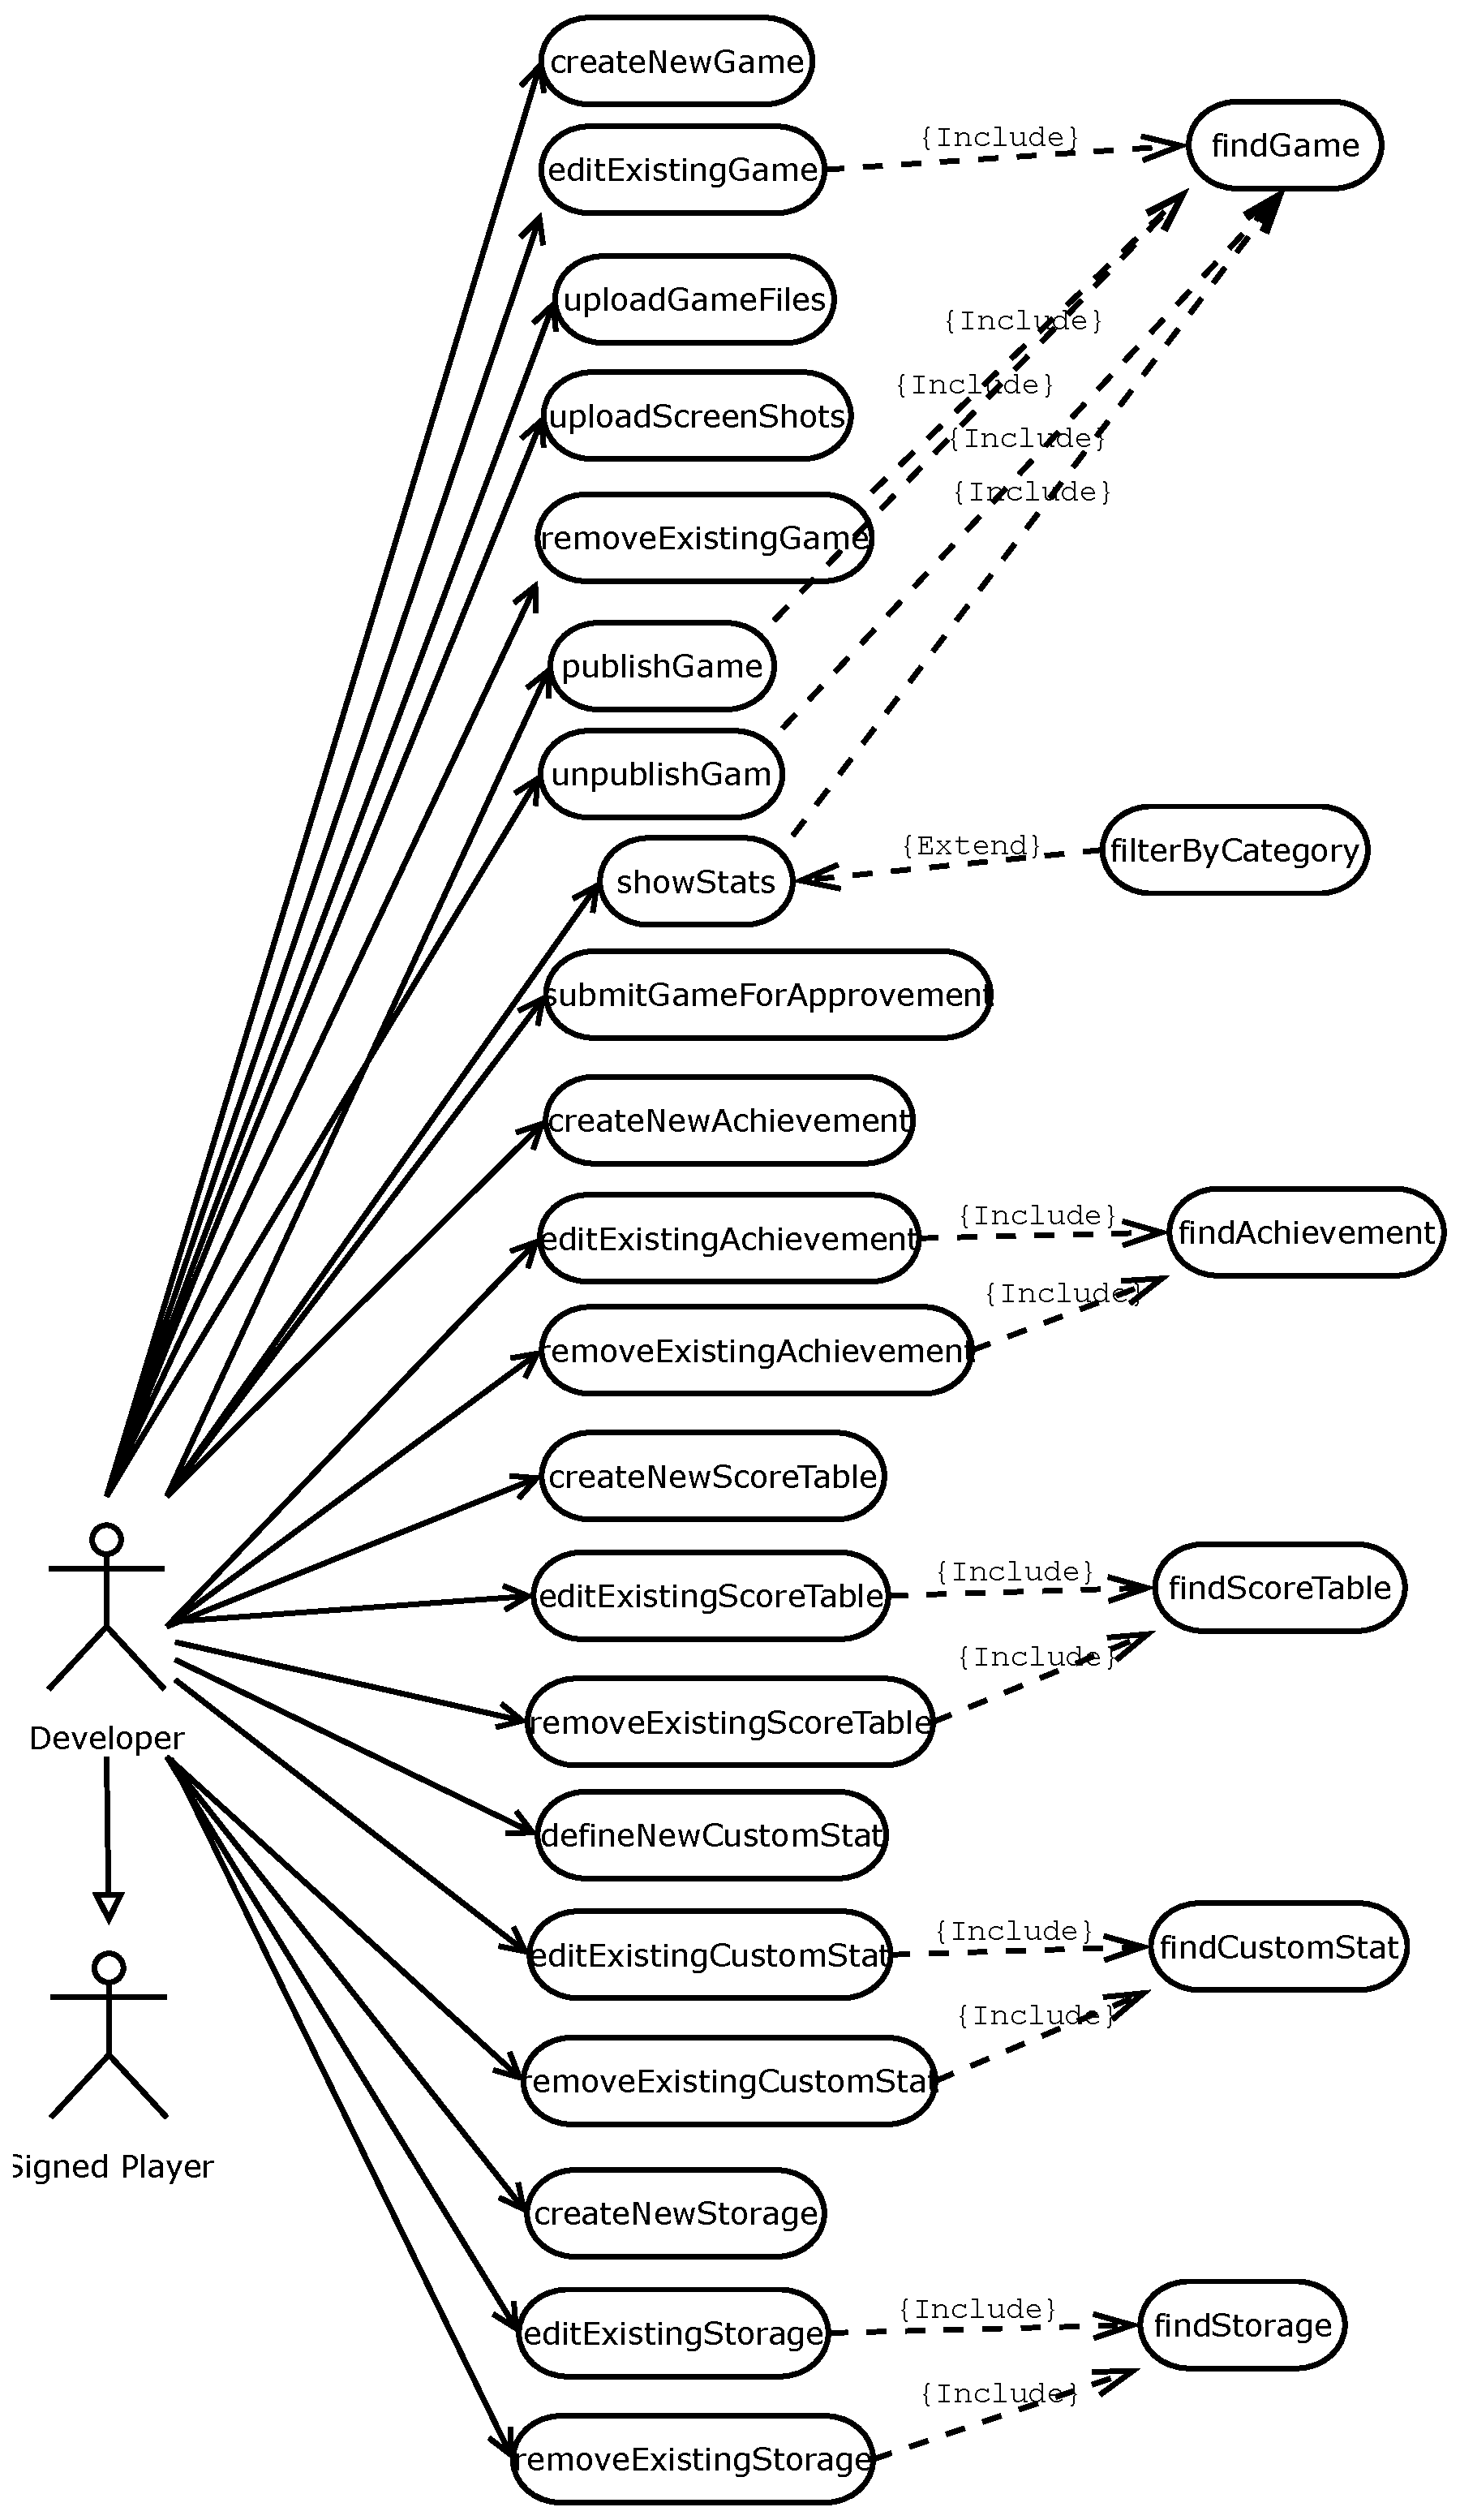
\includegraphics[scale=0.40]{fig/ucd-vyvojar.eps}
  \caption{Use Case Diagram vývojára}
  \label{fig:ucdvyvojar}
\end{figure}
\clearpage

Poslednou, avšak nie nevýznamnou rolou, ktorá sa v pomyslenom hierarchickom rebríčku právomocí nachádza úplne najvyššie, je rola administrátora webovej platformy. Bežný užívateľ nemá možnosť stať sa administrátorom žiadnou akciou z jeho strany. Užívateľa môže povýšiť na administrátora iba iný administrátor, alebo správca databáze, ktorý má prístup k tabuľkám užívateľov a ich rolí. Administrátor má všetky práva a môže vykonávať všetky akcie a riadiť všetky udalosti na platforme, ktoré mu grafické užívateľské prostredie dovoľuje vykonávať. Teda užívateľ, ktorý nadobudol rolu administrátora môže vykonávať všetko to čo neprihlásený návštevník, prihlásený hráč a zároveň aj vývojár. Okrem toho takýto užívateľ má na starosti správny chod platformy, teda by mal mať možnosť deaktivácie a znovu aktivácie užívateľských účtov, v prípade, že by konkrétny užívateľ nejak porušoval pravidlá platformy. Tento užívateľ by mal mať možnosť editácie všetkých hier a všetkých užívateľských profilov, nielen tých, ktoré mu patria. Ďalšou významnou úlohou, ktorú má rola administrátora na starosti, je schvaľovanie a odmietanie vývojármi vytvorených a odoslaných hier na schválenie.
\begin{figure}[h]
  \centering
  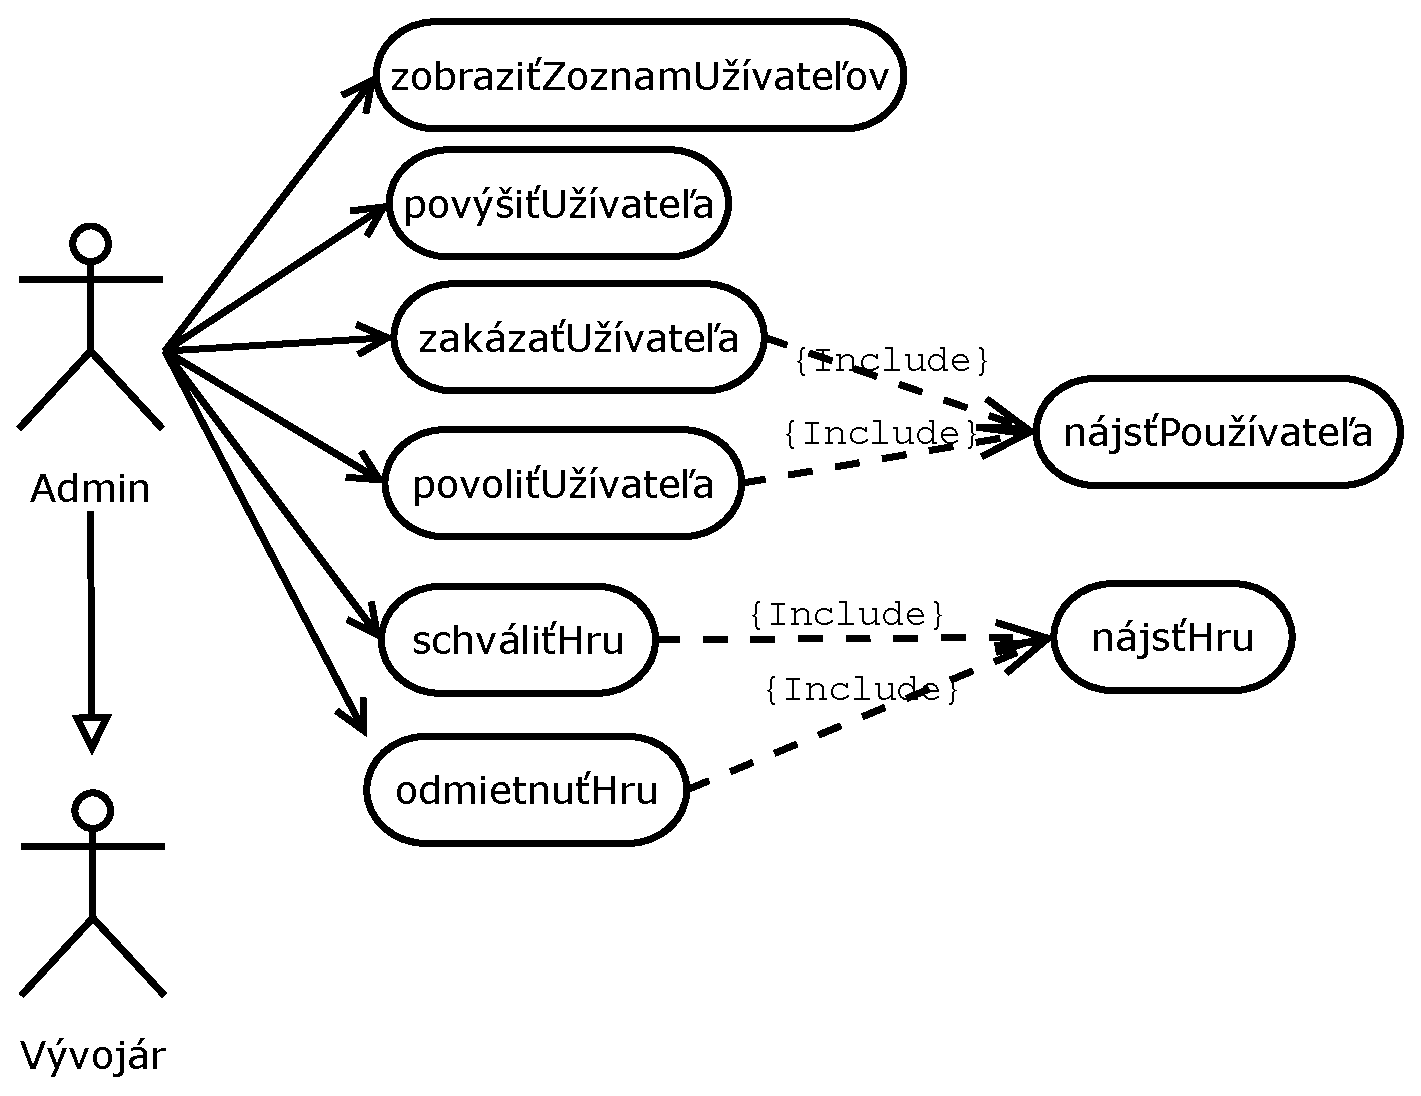
\includegraphics[scale=0.40]{fig/ucd-admin.eps}
  \caption{Use Case Diagram administrátora}
  \label{fig:ucdadmin}
\end{figure}

Návrh grafického užívateľského rozhrania môže byť kľudne rozdelený podľa rolí, teda na stránky, kam pristupuje administrátor, kam zase developer, a kam hráč a návštevník webu. Podľa toho sa dá potom rozhranie správne pripraviť a navrhnúť. V prvom rade je ale dobré si uvedomiť, ktoré prvky majú všetky 3 role spoločné. Určite to bude menu v hlavičke, ktorého návrh môžete vidieť na obrázku \ref{fig:guihlavicka}. Táto hlavička by mala obsahovať nejaké textové, alebo obrázkové logo naľavo a základné menu napravo. Pričom obsah v menu napravo by bol generovaný podľa toho, v akej roli užívateľ vystupuje. V prípade, že nie je užívateľ prihlásený/registrovaný, tak by sa tam mal nachádzať formulár na prihlásenie/registrovanie. 
\begin{figure}[h]
  \centering
  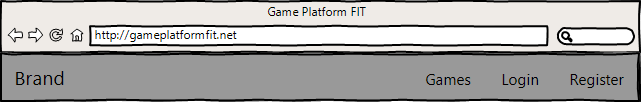
\includegraphics[scale=0.50]{fig/gui-hlavicka.png}
  \caption{Hlavička s logom a menu}
  \label{fig:guihlavicka}
\end{figure}

Stránky určené pre hráčov hier by boli: stránka so zoznamom hier, detail hry a poprípade profil hráča. Stránka so zoznamom hier by obsahovala prirodzene jednotlivé hry. Každá hra by tu bola reprezentovaná názvom a svojím náhľadovým obrázkov, nie snímkou z hry, skôr nejakou graficky príťažlivou upútavkou k hre. Zoznam hier by mal byť filtrovateľný podľa jednotlivých kategórií. Návrh môžete vidieť na obrázku \ref{fig:guihry}.
\begin{figure}[h]
  \centering
  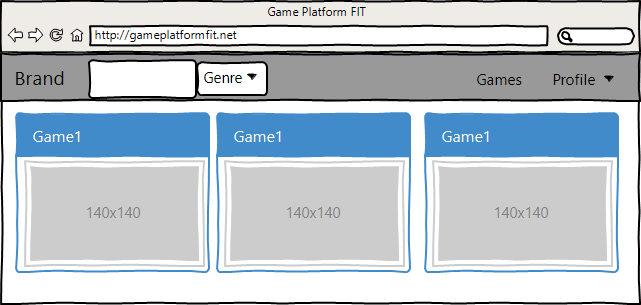
\includegraphics[scale=0.48]{fig/gui-hry.png}
  \caption{Stránka s hrami}
  \label{fig:guihry}
\end{figure}

Detail hry by mal obsahovať slide show obrázkov už zo samotnej hry. Slideshow by sa mala sama meniť poprípade by mal užívateľ možnosť ručne prechádzať obrázky pomocou šípiek na stranách. Ďalej by tam boli základné informácie o hre ako popis a inštrukcie, ktoré by boli zobrazené kvôli grafickej príťažlivosti v paneloch. V rovnakých paneloch by mali byť zobrazené aj odmeny a tabuľky skóre. Prihlásený hráč by mal tiež vyznačené, ktoré odmeny získal, a ktoré nie. Riadok so získanou odmenou by bol vyfarbený na zeleno, s odmenou, ktorú ešte nezískal zase na červeno. Pod tým všetkým by sa malo nachádzať tlačidlo „Play“, slúžiace na spustenie hry. Úplne na konci by sa mali nachádzať pridané komentáre k hre od užívateľov a formulár, kde by samozrejme prihlásený užívateľ mal tiež možnosť komentovať. Celý zjednodušený návrh môžete vidieť na obrázku \ref{fig:guidetailrhy}.
\begin{figure}[h]
  \centering
  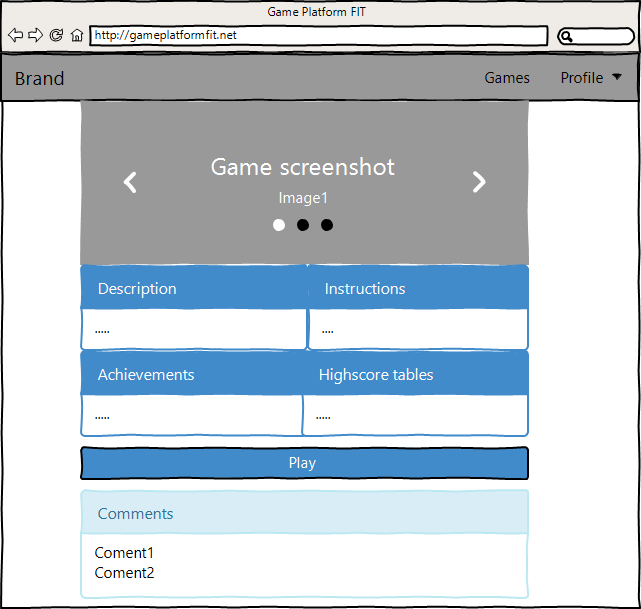
\includegraphics[scale=0.35]{fig/gui-detail-hry.png}
  \caption{Detail hry}
  \label{fig:guidetailrhy}
\end{figure}

Stránky, ku ktorým by pristupoval vývojár hry by boli tie isté, ako stránky, ku ktorým pristupuje hráč. Okrem toho by mal mať prístup do vývojárskej konzole, kde by bol zoznam hier, ktoré daný vývojár vyvíja a detail, alebo lepšie povedané úprava/tvorba existujúce/novej hry. Vývojárska konzola so zoznamom hier by bola takmer totožná z hľadiska GUI ako  už popísaný zoznam hier určený pre hráča, takže ju nemá zmysel popisovať podrobnejšie. Stránka s detailom vyvíjanej hry by pozostávala z panelov. Každý panel by mal slúžiť pre iný druh informácií. Jeden by bol pre hlavné informácie o hre, druhý pre grafické materiály k hre, tretí k odmenám, tabuľkám skóre a zobrazenie štatistík. Informácie v každom paneli by boli editovateľné poprípade vytvoriteľné po kliknutí na tlačidlo „Edit“, po ktorom by sa vyvolalo modálne okno s príslušným editačným formulárom.
\begin{figure}[h]
  \centering
  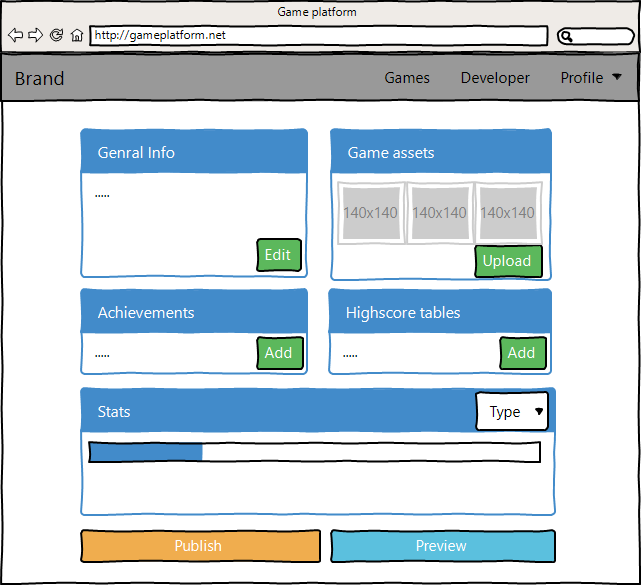
\includegraphics[scale=0.35]{fig/gui-detail-vyvojar.png}
  \caption{Úprava hry v vývojárskej konzole}
  \label{fig:guidetailvyvojar}
\end{figure}

Admin by mal samozrejme prístup ku všetkému v rámci platformy. Teda by mohol využívať stránky navrhnuté ako pre hráča, tak aj pre vývojára hier. Admin taktiež potrebuje nejakú administrátorskú konzolu, aby mohol spravovať hry a užívateľov. Mal by v tejto konzole mať možnosť vidieť hry, ich status, alebo presnejšie povedané, či sú schválené, alebo neschválené a mať možnosť ich jednoducho schváliť, alebo zamietnuť z publikácie. V zozname užívateľov by mal mať zase možnosť jednotlivý užívateľom odopierať prístup na stránku, poprípade prístup povoľovať. Mockup administrátorskej konzole je možné vidieť na obrázku \ref{fig:guiadmin}.
\begin{figure}[h]
  \centering
  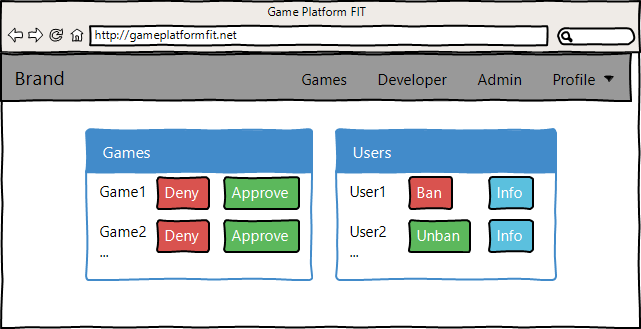
\includegraphics[scale=0.35]{fig/gui-admin.png}
  \caption{Konzola administrátora}
  \label{fig:guiadmin}
\end{figure}

\section{Návrh databáze}
Návrh databáze vychádza v určitej miere z predchádzajúcej kapitoly o návrhu webovej platformy, kde boli predstavené a namodelované diagramy prípadov užitia. Tieto 2 kapitoly teda spolu úzko súvisia, keďže užívateľ chce na webovej platforme vykonávať rôzne akcie a častokrát, alebo aj skoro vždy, požaduje, aby sa informácie niekde uchovali, poprípade aby už uložené informácie od nekaľ získal. Táto kapitola teda do istej miery obsahuje informácie už uvedené v kapitole o návrhu webovej platformy, s tým rozdielom, že informácie sú interpretované tak, aby z nich bolo možné urobiť návrh databázy. Z nasledujúceho popisu by malo vyplývať, aké informácie v databázy je potrebné uchovávať. 

Návrh databáze bol modelovaný pomocou Entity relationship diagram (ERD) s Unified modeling language notáciou. ERD sa využíva v softwarovom inžinierstve pre abstraktné a konceptuálne znázornenie dát. Pri modelovaní takéhoto diagramu vzniká jeden z typov konceptuálnych, alebo schematických dátových modelov systému, v tomto prípade relačnej databáze, a požiadaviek na ňu z hora dole. V prípade že sa jedná o návrh webovej platformy, portálu alebo iného vo svojej podstate informačného systému, ktorý je založený na databázy, tak sa konceptuálny model v neskoršej fázy mapuje na logický dátový model (napríklad relačný model), a ten je ďalej mapovaný na fyzický dátový model. Existuje niekoľko bežných notácií využívaných pre ERD určené pre rôzne typy návrhov, ako logické, fyzické alebo konceptuálne. Jedny zo známych konvencií pre písanie diagramov sú Chenova notácia, Crows Foot notácia alebo už spomenutá UML notácia.

Najhlavnejšiu úlohu v tomto projekte zastáva hra. Hra je teda v diagrame akási centrálna entita, bez ktorej by nemalo zmysel tento databázový návrh, a vôbec celý projekt robiť. Hra obsahuje názov, popis, inštrukcie, ikonu, titulný obrázok, dvojicu kľúčov, aktuálne nahranú verziu hry na portáli, jeden herný žáner a príznaky, či je vyvíjaná, publikovaná, schválená, odmietnutá, a či využíva funkciu uzamknutia na domény. Hra môže mať niekoľko snímok obrazovky, minimálne ale 1 musí byť prítomný vždy. Daný snímok obrazovky patrí vždy jednej konkrétnej hre. Snímok obrazovky obsahuje url, kde sa nachádza v rámci serveru. Ďalej môže byť hre priradených niekoľko domén, daná doména môže prislúchať práve jednej hre. Doména obsahuje svoju url. Hra tiež obsahuje ďalšie funkcie spojené prevažne s API, ako štatistika, vlastná štatistika, cloud úložisko, tabuľky skóre a odmeny. Štatistika prislúcha práve jednej danej hre a hra môže mať niekoľko štatistík. Štatistika v sebe obsahuje informácie o IP adrese, čase, dátume, zemepisnej šírky a dĺžky, štáte, mesta, internetovom poskytovateľovi a použitom internetovom prehliadači. Okrem toho ale hra môže mať definované vlastné štatistiky. Týchto štatistík môže byť hneď niekoľko a daná vlastná štatistika prislúcha práve jednej hre. Vlastná štatistika obsahuje svoje meno a hodnotu. Úložísk môže mať hra taktiež niekoľko a jedno konkrétne úložisko patrí iba jednej hre. Úložisko má v sebe uložené hodnoty, ktorých môže byť viac, jedna hodnota úložiska patrí jednému úložisku a zároveň jednému konkrétnemu užívateľovi. Odmeny obsahujú meno, popis, url obrázku, a body. Daná odmena patrí k jednej hre a hra odmien môže mať viacero. Užívateľ tieto odmeny má možnosť získať a môže ich získať toľko, koľko odmien existuje. Posledným z API tabuliek sú skóre tabuľky. Skóre tabuliek môže mať hra niekoľko a jedna skóre tabuľka patrí k jednej hre. V skóre tabuľke sa nachádzajú hodnoty, ktorých môže mať skóre tabuľka veľa, ale jedna konkrétna hodnota skóre patrí práve jednej skóre tabuľke a zároveň jednému užívateľovi. Užívateľ je ďalšia dôležitá entita, ako je už vidieť z predošlých riadkov. Užívateľ v sebe nesie informácie o svojej prezývke, menu, priezvisku, heslu, e-mailu, biografií, obrázku, o svojej roli v rámci systému a príznak či má zákaz prístupu na stránku, alebo nie. Hra sa môže nachádzať u hocijakého počtu hráčov v ich osobných knižniciach. Táto osobná knižnica v podstate predstavuje zoznam obľúbených hier. Hru by mal mať možnosť užívateľ do tejto knižnice pridávať, v prípade, že sa tam ešte nenachádza, alebo v prípade, že sa tam už nachádza, by ju mal mať možnosť z nej odstrániť. Hráč môže mať vo svojej knižnici hocikoľko hier, alebo v nej nemusí mať žiadnu hru. Užívateľ by ďalej mal mať možnosť hru ohodnotiť a komentovať. Hra môže byť hodnotená a komentovaná od hocijakého počtu prihlásených užívateľov. Užívateľ môže komentovať jednu hru niekoľko krát, avšak hodnotiť ju môže iba raz, a potom môže svoje hodnotenie už iba upravovať. Danú konkrétnu hru môže vyvíjať iba jeden užívateľ.
\begin{figure}[h]
  \centering
  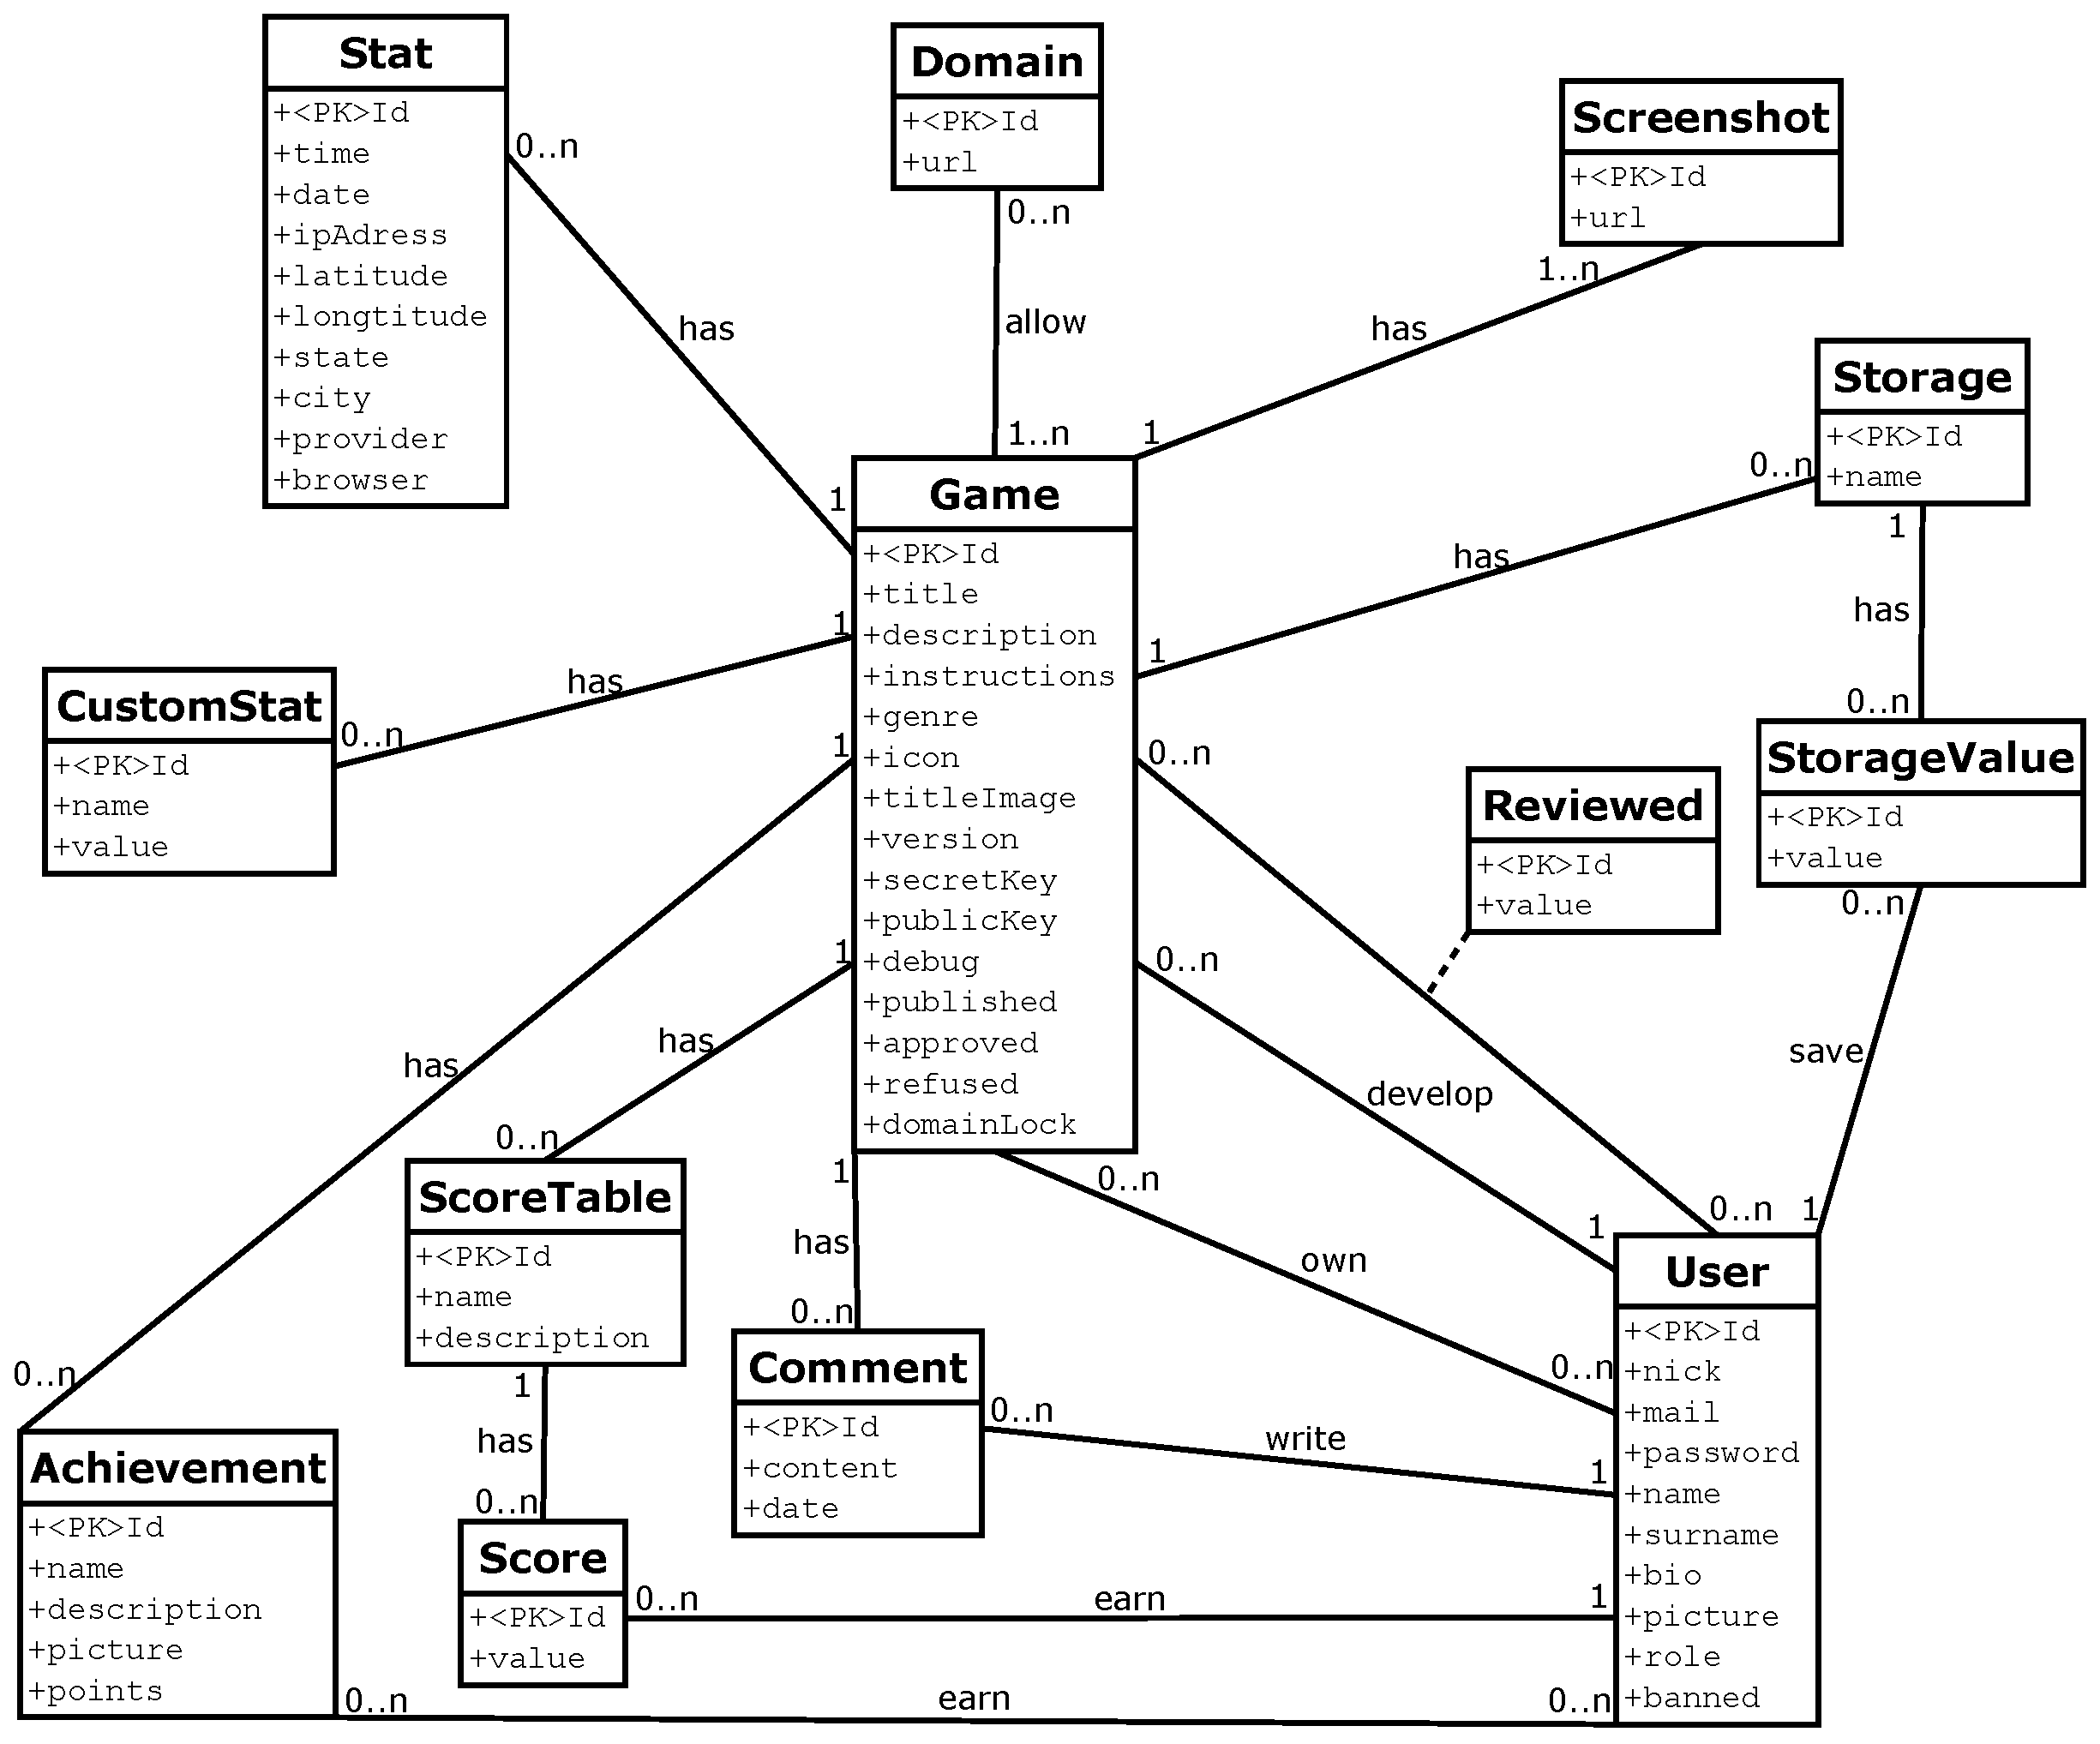
\includegraphics[scale=0.4]{fig/erd.eps}
  \caption{Návrh databáze ako ER diagram}
  \label{fig:erd}
\end{figure}

\section{Návrh API}
API by malo byť implementované z väčšej časti na serverovej strane, z menšej časti na strane klienta. Malo by fungovať tak, že klient inicializuje spojenie so serverom pomocou AJAX a CORS. V XHR správe pošle nejaký identifikátor, pravdepodobne špeciálne vygenerovaný reťazec tzv. API kľúč. Server by mal následne odpovedať, ideálne v nejakom formáte, ktorý server dokáže vygenerovať a klientská strana zase čítať. Na tento účel bol vybraný JavaScript Object Notation, skrátene JSON, ktorý sa používa pre takýto typ prenosu dát. Výhodou je, že je platformne nezávislý, a to aj napriek tomu, že používa Javascriptovú syntax. Server by teda mal odoslať odpoveď o tom, či spojenie akceptuje a preniesť ďalšie potrebné dáta. Odoslaná JSON správa by mala vyzerať tak, že by sa tam nachádzala akási položka status, ktorá by vypovedala o tom, ako skončila operácia vykonávaná na serveri, či skončila úspechom, poprípade neúspechom, a akým presne. 
\begin{lstlisting}[]
{
    status: '0',
    data: 'some data'
}
\end{lstlisting}
Daný neúspech by bol definovaný dopredu určeným číslom. V položke dáta by zase boli klientom požiadané dáta, v prípade že operácia skončila úspechom a tieto dáta by sa na klientskej strane v danej funkcií spracovali do užívateľsky prijateľnej podoby, a následne by boli ďalej predané do aplikácie
\begin{table}[h]
\centering
\begin{tabular}{|l|l|l|}
\hline
Položka status/návratový kód & Význam \\ \hline
0 & Operácia na servery skončila úspešne \\ \hline
1 & Operácia na servery skončila neúspešne \\ \hline
1\textless & Ďalšie, špecifickejšie neúspešné skončenie operácie \\ \hline
\end{tabular}
\label{navratovekody}
\caption{Tabuľka návrhov návratových kódov}
\end{table}

Z vybraných komponent pre použitie v API vyplýva, že by v API mali byť implementované nasledujúce funkcie:
\begin{enumerate}
\item Inicializácia API
\item Meranie štatistík prístupov
\item Kontrolovanie domén
\item Práca s užívateľským účtom
\item Práca s tabuľkou skóre
\item Práca s odmenami
\item Práca s cloudovým úložiskom
\end{enumerate}

\section{Návrh Hry}
Pri tvorbe návrhu hry bolo brané na vedomie, že hra má byť jednoduchá, čo sa týka použitých programovacích techník, keďže hra má slúžiť predovšetkým na demonštráciu webovej platformy a jej API. Vývojár, ktorý by si chcel eventuálne hru rozobrať, by sa nemal snažiť pochopiť príliš zložitý kód. Z toho dôvodu, boli hneď vylúčené zložité herné žánre a na výber sa ponúkali skôr klasické hry (rôzne logické stolné hry, ako pexeso, puzzle...), alebo pomerne nové obľúbené a populárne mobilné casual hry\footnote{Herný žáner cielený na občasných hráčov hier, vyznačujúci sa väčšinou predovšetkým veľmi jednoduchými pravidlami} (napríklad Flappy Bird, TimberMan, alebo rôzne Match3 klony), ktoré sú v niektorých prípadoch na implementáciu ešte jednoduchšie, ako spomínané klasické žánre. Ďalším dôležitý kritériom pri návrhu demonštračnej hry bolo, aby v hre boli implementovateľné všetky navrhnuté funkcie API. Posledným, avšak nie až tak dôležitým kritérium bolo, aby celá grafická stránka hry bola ľahko vytvoriteľná aj pre človeka, ktorý nie je primárne grafikom. Ideálne by teda hra mala byť bez zložitých animácií a ďalších v tomto prípade zbytočných zložitostí.  

Po zhodnotení možností, bolo ako demonštračná hra zvolené pexeso. Dôvodom je to, že pexeso je pomerne ľahko implementovateľné. Dajú sa do neho integrovať všetky navrhnuté API funkcie a pre tvorbu grafiky nie sú potrebné žiadne pokročilé grafické skúsenosti, nehovoriac o animáciách. Hra by sa mala skladať z niekoľkých obrazoviek, z hlavného menu, z obrazovky, na ktorej bude zobrazená tabuľka najlepších hráčov s ich skóre, obrazovka slúžiaca ako akási sieň trofejí, v ktorej budú zobrazené získané odmeny a obrazovka, na ktorej sa bude odohrávať samotná hra. Na obrazovke hry by bola zobrazená hracia plocha + nejaký základný HUD\footnote{Head-up display, metóda, ktorá vizuálne odovzdáva informácie hráčovi, ako súčasť užívateľského rozhrania hry}, informujúci o tom, koľko kariet zostáva otočiť, koľko hráč nahral bodov, a aké je doposiaľ najväčšie nahrané skóre daného hráča. Základný grafický návrh rozloženia hernej obrazovky môžete vidieť na obrázku.
\begin{figure}[h]
  \centering
  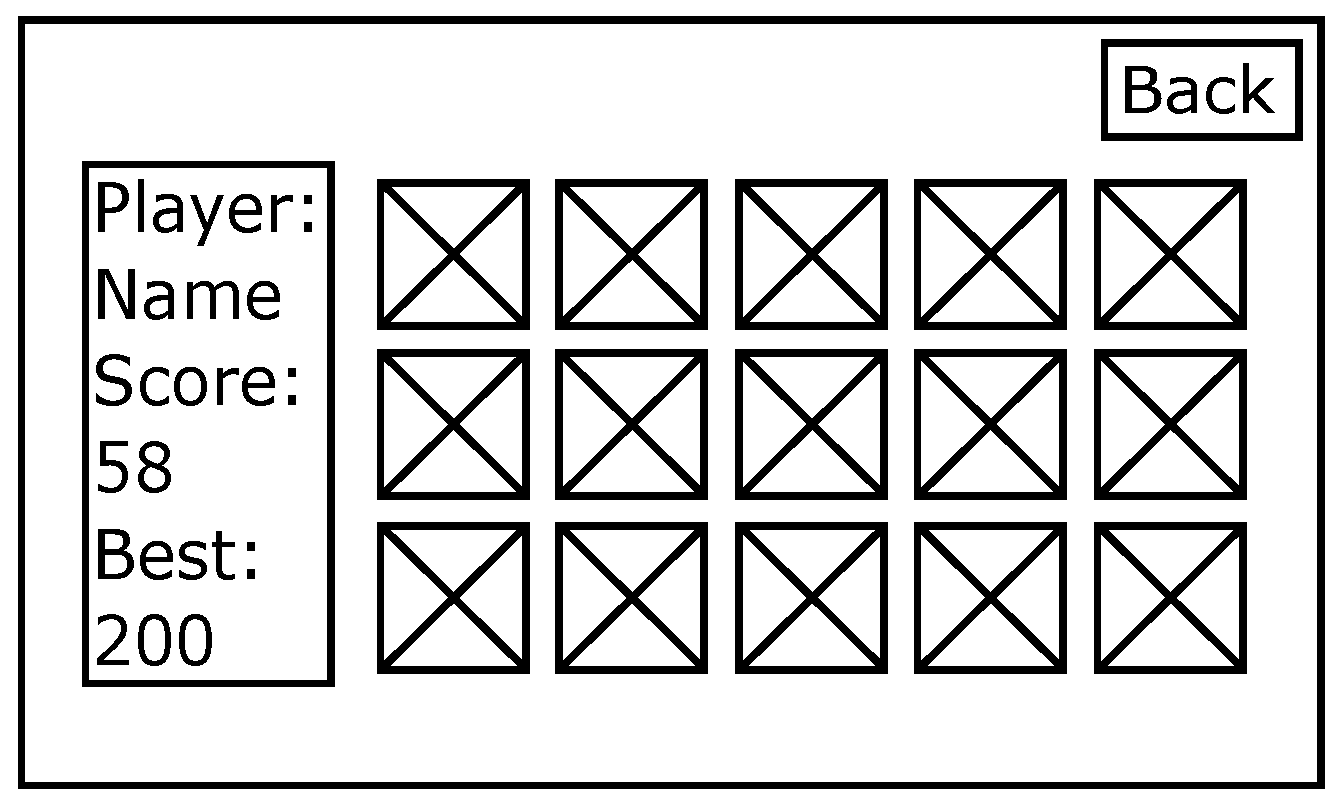
\includegraphics[scale=0.5]{fig/gui-hra.eps}
  \caption{Návrh prostredia hry}
  \label{fig:guihra}
\end{figure}

Hráč má v tejto hre za úlohu nájsť všetky rovnaké dvojice hracích kariet. Ak by našiel rovnakú dvojicu, tak by získal +10 bodov.  Ak by otočil dvojicu rozdielnych kariet v jednom kole, tak by stratil -1 bod. Takto by mohol získavať skóre a následne po otočení všetkých rovnakých dvojíc by jeho skóre bolo odoslané na server a hráč by bol presmerovaný na obrazovku s tabuľkou najlepších hráčov. Odmeny by mohli byť implementované napríklad tak, že ak by hráč otočil 2 rovnaké dvojice 3 krát za sebou, tak by získal odmenu, ak 5 krát, tak by získal ďalšiu odmenu, ak by prešiel celú hru na jeden pokus, tak zase inú odmenu, a tak podobne. Cloudove úložisko by zase mohlo v tejto hre slúžiť, ako počítadlo, koľko hier daný hráč odohral. 

\chapter{Implementácia}
\label{chap:implementacia}
Tak ako kapitola venujúca sa návrhu rešenia bola rozdeleá do logických častí, tak aj táto kapitola pojednávajúca o konkrétnej implementácií je rozdelená do obdobných logických častí. Kapitola začína popisom implementácie wbvovej platformy, pokračuje implementáciou API a končí implementáciou hry.  Každá táto časť popisuje podrobnejšie významné implementačné detaily, ktoré boli navrhnuté v kapitole o návrhu riešenia. 

\section{Implementácia webovej platformy}
todo

\section{Implementácia API}
todo

\section{Implementácia demonštračnej hry}
todo

\chapter{Testovanie}
\label{chap:testovanie}
todo

\chapter{Záver}
\label{chap:zaver}
todo












%=========================================================================
